\documentclass[a4paper,11pt]{report}


\usepackage[utf8]{inputenc}
\usepackage[T1]{fontenc}
\usepackage{lmodern}
\usepackage[norsk]{babel}
\usepackage{parskip}
\usepackage{graphicx}
\usepackage{caption}
\usepackage{subcaption}
\usepackage{titlepic}
\usepackage{a4wide}
\usepackage[htt]{hyphenat}
\usepackage{enumitem}
\usepackage{color}
\usepackage{hyperref}
\usepackage{listings}
\usepackage[section]{placeins}
\lstdefinestyle{java1}{
  language=Java,
  basicstyle={\ttfamily\footnotesize},
  numberstyle={\ttfamily\footnotesize},
  keywordstyle={\ttfamily\footnotesize\color[rgb]{0,0,1}},
  commentstyle={\ttfamily\footnotesize\color[rgb]{0.133,0.545,0.133}},
  stringstyle={\ttfamily\footnotesize\color[rgb]{0.627,0.126,0.941}},
  breaklines=true,
  columns=fixed,
  extendedchars=true,
  numbers=left,
  numbersep=3pt,
  showspaces=false,
  showstringspaces=false,
  stepnumber=1,
  tabsize=2
}
\lstset{style=java1,
literate=%
{æ}{{\ae}}1
{å}{{\aa}}1
{ø}{{\o}}1
{Æ}{{\AE}}1
{Å}{{\AA}}1
{Ø}{{\O}}1
}
\renewcommand\lstlistingname{Eksempel}
\renewcommand\lstlistlistingname{Eksempler}

\usepackage{fancyhdr}
\setlength{\headheight}{15.2pt}
\pagestyle{fancy}
\fancypagestyle{plain}{ %
  \fancyhf{} % remove everything
  \renewcommand{\headrulewidth}{0pt} % remove lines as well
  \renewcommand{\footrulewidth}{0pt}
}

%Her kommer opsett av info for pdf filen
%\pdfinfo{%
%  /Title    (Rapport prosjektoppgave i programutvikling)
%  /Author   ()
%  /Creator  ()
%  /Producer ()
%  /Subject  ()
%  /Keywords ()
%}



\begin{document}
\begin{titlepage}
%\begin{center}
 



\title{Servicios De Vivienda}

\titlepic{
\includegraphics[width=40mm]{./img/fremside/logo.jpg}}

\author{Espen Zaal\\Lukas Larsed\\Petter Knagenhjelm Lysne}
\date{\today}



%\end{center}
\end{titlepage}

\maketitle
\begin{abstract}
\lettrine[lines=3]{Å} summere to måneders hardt arbeid ned på en side eller to er vanskelig. Det begynte ganske så greit. Det var en god del diskusjoner den første tiden på hvordan programmet skulle se ut. Spesielt dette med at vi må simulere en virkelighet der man ser for seg boligsøker som sitter hjemme og søker etter boliger, og megler har kontrollen på resten. Det var litt vrient å velge hvordan man skulle tolke oppgaven sånn sett. Den ga mye frihet, og resultatet vi har kommet frem til nå mot slutten er helt annerledes enn det vi opprinnelig skisserte i de første tegningene.

Vi endte opp med en løsning der boligsøker utfører søkene sine i sitt panel, og om en finner en interessant annonse så kan en søke på den. Boligsøker må bekrefte utleier sine krav for boligen før søknaden havner i søknadslisten hos megler. Megler på sin side har myndighet fra utleier til å både opprette boligobjektene og annonsene, samt godkjenne den søknaden han mener er det beste alternativet. Megler skriver så kontrakt med rett boligsøker, på vegne av utleier.

På et tidspunkt før vi begynte selve utviklingen satt vi av en god uke der vi hver for oss skulle lære så mye om \texttt{Swing} som mulig. På de tidspunktet hadde vi ikke nok grunnkunnskap om hva som er mulig rent teknisk og hva vi realistisk kunne få til innenfor tidsrammen.

MVC-arkitektur ble raskt besluttet at vi skulle ha. Skrekkhistorier om java-filer på flere tusen rader, samt at ingen av dem ville kunne gjenbrukes var ikke fristende. Dette var en stor inspirasjonskilde for videre læring og utvikling. Vi ble raskt vant til å finne flere kilder til informasjon enn bare pensum, da våre utfordringer ofte lå godt utenfor pensum.

MVC er egentlig lagdelt arkitektur. Datalaget, brukergrensesnittet og logikken, hver for seg i forskjellige lag, der logikklaget styrer all funksjonalitet. Bare ved å ha de samme to kontrollerne \texttt{ControllerTabell.java} og \texttt{ControllerOutput.java} til å virke både i meglervindu og annonsevindu har vi spart ca 2000 kodelinjer, samt betydelig med tid i forhold til å slippe å oppdatere samme funksjonalitet flere steder.
Når vi nå nærmer oss slutten på prosjektet, har vi dekket hele oppgavens krav om implementasjon av teknologi, men samtidig lagt til rette for å kunne utvide programmet videre.

Ser man på selve gruppearbeidet og prosessen vår som gruppe, så er det en del lærdom å ta med seg derfra. Det krever mye erfaring å få en gruppe til å være mest mulig produktiv. Å fordele oppgaver som både gir mening og som tar prosjektet fremover er vanskelig, og da alle i gruppen lærte mye av de tekniske underveis, ble det ikke så effektivt som ønskelig.

Om en skal summere prosjektet som helhet, er alle i gruppen fornøyde med resultatet. Allerede nå ser vi forbedringer man gjerne skulle gjort om man hadde hatt tid, eller kunne begynt på nytt, men kompleksiteten av de vi har implementert og mengden funksjonalitet som er implementert er vi godt fornøyd med.




\end{abstract}
\chapter*{Om programmet}
Her følger en liste over utvalgte egenskaper ved programmet vårt.

\textbf{Strukturelle egenskaper og detaljer}

\begin{itemize}[noitemsep,nolistsep]
\item Det er brukt \texttt{MVC}-arkitektur gjennom hele programmet. Ingen vinduer kjenner til datastrukturen og omvendt. \\
\item Det har vært hovedfokus på gjenbruk av kode. Det er skrevet veldig få metoder i flere klasser som utfører samme type jobb. \\
\item Vi har laget egendefinerte \texttt{Swing}-komponenter som har utvidet funksjonalitet. Feks \texttt{CustomJTextField} med innebygget \texttt{RegEx}-tester. \\
\item Det er brukt arv i flere nivåer, spesielt i brukergrensensittet, men også i datamodellene. \\
\item Det brukes egenlagde \texttt{interface-lyttere} som muliggjør kommunikasjon mellom klasser som ellers ikke har tilknytning til hverandre. \\
\item Vi har brukt klasser som hovedpaneler i stedet for én GUI-klasse med flere "\texttt{JPanels}". Dette for å kunne bytte ut et "toppanel" eller "bunnpanel" ved senere behov, uten at hele programmet berøres. \\
\item De to arkfanene er bygget på samme \texttt{Layout}, og deler \texttt{kontrollere} og funksjonalitet. \\
\item Omfattende bruk av egendefinerte \texttt{static} konstanter som kalles opp for å sette vindustørrelser, komponentfarger osv. \\
\item Login-løsning for megler. En kan ikke komme inn i det panelet uten å logge seg på. \\
\item I det man oppretter en bolig, opprettes også en mappe på datamskinen. Om ikke bilder legges til boligobjektet så får den med et standardbilde. Andre bilder man legger til havner i denne nye mappen.\\\\
\end{itemize}


\textbf{Tekniske egenskaper og implementasjoner}

\begin{itemize}[noitemsep,nolistsep]
\item Bruk av \texttt{JTable} med egne \texttt{TabellModeller} som arver \texttt{DefaultTableModel}. Tabellen har også to forskjellige sorteringsmetoder, en \texttt{CustomCellRenderer} og automatisk kolonnebreddejustering. \\
\item Alle objekter vises i \texttt{HTML}-format i en \texttt{JEditorPane}. \\
\item Egenlaget fritekstsøk ved hjelp av å implementere et \texttt{interface} på de objektene som skal søked gjennom. \\
\item Bruk av \texttt{generiske} datatyper og metoder både ved fritekstsøket og i datastrukturen.
\item PopupMeny ved høyreklikking i tabellen. \\\\
\end{itemize}


\textbf{Egenskaper i brukergrensesnittet} \\

\begin{itemize}[noitemsep,nolistsep]
\item I det man velger et objekt i tabellen vil knappene i toppanelet aktivere/deaktivere seg ettersom hvilke valg man skal kunne ta. Man må velge en utleier før man kan opprette ny bolig. \\
\item Dobbelklikk på et objekt i tabellen vil åpne det objektets registreringsvindu med ferdig utfylt data som kan endres. \\
\item Høyreklikk på et objekt i tabellen vil gi en utvalgt popupmeny med bare de valg som gjelder for denne typen objekt. \\
\item En kan slette objekter fra tabellen ved å trykke på Delete-knappen på tastaturet. En kan ellers få dette valget i popupmenyen. \\
\item Når en har valgt et annonseobjekt så kan en klikke i "utskrifts-vinduet" for å få opp en bildeviser er en kan bla gjennom flere av annonsens bilder. \\
\item Det er tastaturkommandoer for å kunne opprette nye objekter uten å bruke mus. \\
\item En kan bruke tabulator mellom alle felter i registreringsvinduene. \\
\item En kan ikke slette boliger som er utleid \\
\item En kan ikke slette utleiere som har boliger registrert hos seg. \\
\item Alle utleiere vil i utskriftsvinduet har en liste over boliger de har registrert. \\
\item Alle Leietakere vil ha en liste over boliger de har vist interesse for. \\
\item I det en boligsøker søker på en annonse vil ikke Leietakerobjektet registreres i registeret. Først når en søknad godkjennes vil Leietakerobjekter havne i personregisteret. \\
\item Når megler godkjenner en søknad, og det ligger 4 andre søknader på samme annonse i listen, så vil de bli markert som "behandlet" og "ikke godkjent" og "grået ut". \\
\item Søknadslisten vil alltid vise ubehandlede søknader øverst, sortert innad på AnnonseID. \\
\item Tabellen er responsiv. Det vil si den oppdatere seg automatisk ved endringer av innhold. \\
\end{itemize}
\tableofcontents
\lstlistoflistings
\listoffigures

%Her kommer alle linker til våre kapitel

\chapter{Introduksjon}
\section{Om rapporten}
Denne rapporten består av flere kapitler som kan leses hver for seg og som har hvert sine formål.

Introduksjonen vil gå gjennom litt av forutsetningene for oppgaven, målene vi har satt oss, tolkningen av oppgaven og valgene vi har tatt på bakgrunn av det. 

Prosessdokumentasjonen vil beskrive aspektet ved arbeidet vårt. Hvordan vi kom sammen som en gruppe, bestemte oss for fremgangsmåte og utfordringene vi har stått overfor underveis.

Produktdokumentasjonen er av det veldig tekniske slaget. Det er gitt mange illustrasjoner og kodeeksempler på utvalgte metoder og funksjonalitet, slik at det skal være overkommelig for utenforstående å sette seg inn i programmet.

Testrapporten vil beskrive de tester vi har utført, hvordan vi har utført dem og hvilke resultater de gav. 

Brukerdokumentasjonen vil både være inkludert i dette dokumentet, samt som et frittstående dokument. Den dokumentasjonen vil gi brukeren oversikt over hvordan en bruker programmet og hvilke muligheter programmet gir.

\section{Beskrivelse}
Lage et datasystem som kan håndtere boligformidling i utleiemarkedet. Utleiere skal få sine tilbud presenter og ha mulighet til å nå potensielle leietakere. Boligsøkende skal kunne registrere sine opplysninger og sende inn ønsket bolig som finnes tilgjengelig for utleie. Firmaet skal registrere alel leieforhold som opprettes slik at boligen og leietakeren ikke lenger vil være registrert som henholdsvis ledig boligsøkende. 

\section{Tolkning av oppgaven}
Med hensikt å klare gjennomføre prosjektoppgave på den tid som vi har tilgjengelig har vi valgt og gjøre noen tolkninger og tilpasninger. I følgende seksjoner følger en beskrivelse av hver enkel punkt som er tilpasset etter hva vi anser er gunstig for å løse oppgaven.
Oppgaven gir oss stor frihet til å prioritere hva som skal implementeres, og noen ting som kanskje ville vært naturlig å ha med, er kanskje ikke tatt med. Dette har vi likevel prøvd å legge til rette for ved en fremtidig utvidelse av programmet. 
Et eksempel på dette er statistikk. Vi har laget \emph{Calendar}-felter i Annonse-objektet som er tenkt brukt i forbindelse med hvor lenge en annonse har vært annonsert, hvor mange dager det tok før den ble utleid osv. Vi har ikke fått implementert en god nok statistikkmodul som tar i bruk dette grunnet tidsmangel.

Vår prioritering har i hovedsak vært rettet mot å lage et så robust program som mulig fra bunnen av, slik at man enkelt kan bytte ut/bygge om store deler av programmet uten at andre funksjoner og funksjonalitet skal merke det.
Mye av tiden vi har brukt på utvikling har dermed gått til å finne de beste strukturelle løsningene, selv om det har vært mer tidkrevende og tilsynelatende ikke vises i det kjørbare programmet. 
Dokumentasjonen vil derfor fokusere mye på de ulike løsningene vi har valgt og hvorfor vi har gjort det slik.

\subsection{Brukergrensesnitt}
Et slik program skulle normalt bli delt opp i to separate kjørbare filer eller programmer, slik at man fullstendig avgrenser grensesnittet for megler og boligsøker. Med tanke på at data fra programmet skal seriaslieres til disk ved avslutning av programmet skulle slik løsning medføre store utfordringer da to uavhengige programmer deler på samme register. For å enkelt demonstrere mulighetene har vi derfor valgt å sette opp begge deler av programmet i et og samme brukergrensesnitt. Grensesnittet for megler og utleier er derfor delt opp i samme vindu med \emph{tabpanes}. 

\subsection{Boligøskere} \label{sec:sokere}
Til forskjell fra det som står i oppgaven har vi valgt å ikke registrere opplysninger til en boligsøker før den bestemmer seg for å melde sin interesse for en bolig. Boligsøker skal i sitt brukergrensesnitt blir presentert med alle tilgjengelige boligannonser skal filtrere utfra egne kriterier. Dersom man ønsker å søke på en bolig vil søkeren bli presentert med en dialog for å legge inn sine opplysninger og sende dem til ansvarlig megler. Før søkeren kan registrere sine opplysninger vil han bli presenter med eventuelle krav fra utleier gjeldende den boligen (feks at det ikke er lov til å røyke). Søkeren må akseptere kravene for å sende en forespørsel. En boligsøker kan søke på flere annonser, og leietakerobjektet blir lagt med som parameter i søknadsobjektet, men ikke registrert i personregisteret før en søknad er godkjent av megler. Denne boligsøkeren vil da ikke kunne søke på flere boliger, da leietakerobjektet er opprettet i personregisteret. 
%\\
%\marginpar{Notat}
%\textit{
%Husk at legge til å ting som vi ikke har implementert at i et riktig program så hadde vi kanskje lagt inn funksjon slik at en boligsøker kan sette opp prioritet og feks søke på tre bolige samtidig men man da må velge hvilken av disse boliger skal være på plass 1, 2, 3. Slik vil da søker unngå vente på svar før man kan søke igjen uten det gir megler fullmakt å gå videre til valg 2 dersom man ikke blir akseptert på valg 1 osv.}

\subsection{Meglere}
I oppgaveteksten står det:
\textit{"<...Ved å matche ledige boliger mot de boligsøkandens beskrivelser skal firmaet informare sine kunder om aktueller leietakere og boliger...">}

Som beskrevet i \ref{sec:sokere} har vi valgt å legge slik matching av boliger på selve søkeren etter en løsning der megleren skal ha slik ansvar er mer fra tiden da datamaskiner ikke var tilgjengelige for publikum. Slik tilpasninger gjør at megleren har i stort sett følgende ansvarsområder som kan håndteres via programmet: (1) registrering av nye utleiere, (2) registrering av boliger som tilhører utleierne, (3) legge ut annonser slik at de blir tilgjengelige for boligsøkere, (4) håndtere innkomne forespørsler, (5) opprette kontrakt mellom søkere og utleiere ved inngått avtale. 
Vi har tolket de slik at megleren har egentlig tilgang til følgende registre:
%Kan brukes for mindre avstand
%\begin{itemize}[noitemsep,nolistsep]
\begin{itemize}
\item Søknader
\item Annonser
\item Utleiere
\item Leietakere
\item Kontrakter
\end{itemize}
Det medfører at megleren vil arbeide med disse registre hvilket tar oss til søkefunksjonen. Avhengig av hva megler ønsker å finne i hvert av disse registrene skal han/hun ha mulighet til å avgrense i hvilket register man ønsker å søke. Slik tilpasning der vi deler opp programmet etter slike registrer gjør det met intuitivt for brukeren og gjør det enklere også for utvikleren.

\subsection{Historikk}
Dersom en leietaker inngår et kontrakt blir sendt med som parameter, sammen med Boligobjektet og Meglerobjektet til et kontraktobjekt. I kontraktregisteret skal det ikke være mulig for megler å foreta sletting slik at data over hvilke boliger ble utleide når til hvilke leietakere. Dette vil da utgjøre historikken som vil være søkbar, selv etter at en eventuelt bolig eller leietaker ikke lenger finnes i andre registre.

\subsection{Utleiere}
En utleier kan ha en eller flere boliger men kan også være en representant i form av en firma. I slik fall har vi mulighet å registrere en utleier som er en kontaktperson men også er en representant for en firma som leier ut boliger. En utleier kan be om å bli slettet fra registeret, men ikke om han har boliger i boligregisteret. 

\subsection{Boliger}
Vi går ut fra at boliger som registreres til utleie er eiendomsobjekter som kan være tilgjengelige på utleiemarkedet så snart et leieforhold er over (dersom slik funksjonalitet ønskes av utleieren). Derfor har vi valgt å legge til funksjonaliteten i boligregisteret å sette opp dato fra hvilket en bolig kan vøre tilgjengelig for utleie på nytt. Eventuelle bilder som blir lagret for boligen følger derfor boligobjektet og ikke annonsen slik at megleren ikke trenger å legge ut bildene på nytt dersom boligen skal plasseres på markedet igjen. En bolig som er utleid kan ikke slettes fra boligregisteret.


\section{Mål}
Følgende mål ble satt opp ved begynnelsen av arbeidet med oppgaven:
\begin{description}
\item[Robusthet]
Det var viktig at vår kode skulle være så generell så mulig slik at vi enkelt kan innføre eventuelle tillegg eller endringer i programmet med den hensikt at kodebasen blir enkel å vedlikeholde. Koden skal derfor bygges opp med hjalp av arv og polyformisme i så stor grad som mulig. Det skal være lite bruk av parametere eller identifikatorer som låser komponenter annet enn i konstanter som skal være låst.
\item[MVC]
Programmet skal være bygget opp etter MVC\footnote{eng. Model View Controller}-arkitektur slik at logikk og brukergrensesnitt er helt avskjermet fra hverandre og all informasjonsutveksling blir håndtert via en kontroller. \\
Det skal være så mye gjenbruk av kode som mulig. De metoder og variabler som kan være \texttt{static} skal være det.
\item[Intuitivt brukergrensesnitt]
Brukergrensesnittet skal være enkelt og oversiktlig slik at en bruker som ikke er kjent med programmet kan foreta boligsøk og sende forespørsel til meglerfirmaet. En ny megler skal rask starte opp i sin modul og på kort tid kunne bli kjent med programmets funksjonalitet.
\item[Faglig utfordring]
Det var et mål at vi strakk oss langt i forhold til å komme opp med løsninger som ikke bare løser oppgaven i henhold til pensum, men på en måte som er mest mulig slik vi tror at man ville gjort det i næringslivet. Det vil si å ikke ta snarveier, velge \texttt{JTable} foran \texttt{JList}, bruke \texttt{MVC}, osv.
\end{description}

\section{Tekniske detaljer}

\subsection{Utviklingsmiljø}
Prosjektet er utviklet i NetBeans og Eclipse IDE\footnote{eng. Integrated Development Enviroment}. Ikoner og annen grafikk er oprettet eller editert i Gimp\footnote{The GNU Image Manipulation Program}. Generelle ikoner er oprettet og lastet ned fra \href{http://www.flaticons.net}{flaticons.net}.

\subsection{Krav til programvare}
Programmet er kompilert med \texttt{javac 1.7.0\_51} og testet på tilsvarende java versjon (\texttt{OpenJDK Runtime Environment}). Programmet er utførlig testet på Linux (Ubutnu 12.04 64-bit, Fedora Core 20 64-bit) samt Mac OS X. Det er gjennomført tilsvarende standard funksjonstester på MS Windows 7 og 8.1 (64-bit) for å versifisere platformuavhengighet. 

\subsection{Versjonshåndtering}
Til versjonhåndtering bruktes GIT via terminal og innebygd støtte i utviklingmiljøer (IDE). Lagring av prosjektet ble gjennomført sentralt via en repository på github. Repository for gruppen er privat frem til innlevering av prosjektoppgaven og kommer til å gjøres tilgjengelig for publikum etter at deadline for prosjektet har utløpt. Kildekoden vil da være tilgjengelig fra følgende linker:

\begin{description}
\item[Kildekode]
\hfill \\
\url{https://github.com/CervecerosCodigo/ServiciosDeVivienda}
\\Lagret som NetBeans Java SE prosjekt.

\item[Rapport]
\hfill \\
\url{https://github.com/CervecerosCodigo/ServiciosDeViviendaInforme}
\\ \LaTeX{} kode
\end{description}
\chapter{Prosessdokumentasjon}
Kapitlet inneholder dokumentasjon over utviklingsprossen og beskriver i detaljert tilnærmingsmåte valgt av gruppen.
Det er ikke brukt mye tid på hvem som har gjort hva, og til hvilken tid. Vi har heller delt det opp slik at vi skriver om hvorfor vi har gjort som vi har gjort, hvilken utfordringer vi støtte på underveis. 

Både prosessdokumentasjonen og produktdokumentasjonen er full av referanser til de kapitlene og seksjonene der man kan lese mer om de forskjellige løsningene, og kodeksempler på hvordan det er løst.
\section{UML}
For å visualiser samspill mellom grunnleggende klasser og datafelt i programmert ble det tegnet opp et UML-diagram over grunnleggende register klasser (se vedlegg \ref{appendix:diagram} figur \ref{fig:uml_diag}, side \pageref{appendix:diagram}). Ut fra UML diagrammet ble det generert kodeskjelett til disse klassene, som utgjorde starten på prosjektet. Følgende klasser er satt opp i UML:
\begin{itemize}[noitemsep,nolistsep]
	\item \textit{abstract Person}
		\begin{itemize}
			\item Megler
			\item Utleier
			\item Leietaker
		\end{itemize}
	\item \textit{abstract Bolig}
		\begin{itemize}
			\item Enebolig
			\item Leilighet
		\end{itemize}
	\item Annonse
	\item Søknad
	\item Kontrakt
\end{itemize}



\section{Arkitektur}
Programmet arkitektur bygger helt på \textit{Model View Controller} filosofi. Detter medfører at all logikk og grafiske brukegrensesnitt er helt separiert fra hverandre i egne moduler og pakker. All kommunikasjon mellom disse håndteres gjennom dedikerte kontrollere og interface. Denne arkitekturen ble valgt tidlig i prosjektet med hensikt på at holde koden så robust som mulig, slik tilnærmig gav oss mulighet til feks. kun inlkudere swing komponenter og kode som tilhører oprettelse av vinduer i egene klasse. All logikk som håndterer funksjoner til grafisk grensesnitt for et enkelt vindu finnes i en egen klasse. Dersom MVC ikke ble brukt for prosjektet hadde det resultert i meget store klasser mest sannsynlig som består av flere tusen rader per vindu. MVC gav oss mulighet til å rask legge til nye funksjoner til en alerede eksisterende vinduklasse. Et godt eksepel på dette er dersom samme vindu skal brukes både for registrering og editering av samme opplysninger. MVC stiler kun krav på at kontrolelren har to kontruktører, en som setter opp vinduet dersom det skal foretas en registrering og en konstruktør som kan brukes for endringer. Denne vil da oprette vindu og hente inn all nødvendig data fra objektet (model). 
\section{Arv og polymorfisme}
I prosjektet ble det benyttet arv og polymorfisme i stor utstrekning med tanke på å gjenbruke så mye kode som mulig. Dette følte vi var krav for å lage et produkt med robust kode der alle moduler er separert fra hverandre. Samtidig har man veldig god kontroll på hva som må endres eller utbedres ved videre utvikling. Mye av komponentene vi bruker har utspring i én, eller veldig få superklasser, og ved endring av disse kan vi forandre store deler av programmet på en enkel måte.

Både personobjekter og boligobjekter har flere subklasser. Det samme har tabellens tabellmodell. Her brukes \texttt{instanceof} for å sjekke hvilken type objekter man har med å gjøre.

\subsection{Swing componenter}
Prinsippet for arv er i størst utstrekking brukt ved GUI-komponenter. De komponentene som ble oftest gjenbrukt ble redefinert i form av abstrakte klasser eller laget som "<Custom">-komponenter. Eksempel på dette er \texttt{JPanel, JTextField} eller \texttt{JButton}. Ved å la disse custom-komponentene arve de opprinnelige komponentene fra \texttt{Swing} kunne vi implementere en custom-komponent i stedet, og dermed raskt raskt endre alle de tilsvarende komponentene utseende og funksjon fra en sentral plass i programstrukturen, insteden for \textit{"<refactoring">} av komponentens definisjon over programmets alle filer.
Omtrent ingen komponenter brukes direkte fra \texttt{Swing} uten først å ha blitt tilpasset for gjenbruk flere steder.

\subsection{Pakkefordeling}
Programmet ble grundig delt opp i forskjellige pakker med tanke på å gruppere tilhørende komponenter sammen, og adskille dem fra komponenter som ikke logisk sett hører sammen. Dette er gjort spesielt med tanke MVC arkitektur. For eksempel alle klasser som bygger opp vinduer er plassert i \texttt{view}-pakke, deretter alle klasser som bygger opp registrerings vinduer er plassert \texttt{view.register}-pakken. For å gjenspeile denne analogien på controller-siden har vi lagt dem respektivt i \texttt{controller}-pakken og \texttt{controller.register}-pakken. Deretter ble alle klasser som \texttt{Person} eller \texttt{Bolig} lagt i pakken \texttt{model}. For grundig beskrivelse av fordeling av pakker og filer, se produktdokumentasjon avsnitt \ref{sec:klasserogpakker} side \pageref{sec:klasserogpakker}.

\subsection{Konstanter og enum}
Konstanter ble brukt med tanke på å ha en sentral definisjon av data som feks. konfigurasjoner. En sentral plassering av konstanter som \texttt{RegEx} eller dimensjoner for \texttt{swing}-komponenter gir mulighet til å sette og hente definisjoner til komponentene vi bruker fra en sentral plass. Enum-typer brukes spesifikt for å sette faste definisjoner angående et spesielt objekt. Et godt eksempel på dette er \textit{sivilstatus} der vi fyller opp en comboboks med enum-verdier i stedet for strenger. 
\section{Arbeidsfordeling}

\begin{table}[ht!]
\caption{Arbeidsfordeling mellom gruppemedlemmer}
\label{tab:arbeidsfordeling}
\begin{tabular}{|p{6.8cm}|c|c|c|}

\hline
Utført av					&Espen&Lukas	&Petter\\ \hline
Dokumentasjon				&$\bullet\bullet\bullet$&$\bullet\bullet\bullet$&$\bullet\bullet$\\	\hline
UML							&$\bullet$&$\bullet\bullet\bullet$&$\bullet$\\ \hline
Main kontroller				&$\bullet\bullet\bullet$&$\bullet$&$\bullet$\\ \hline
GUI-struktur					&$\bullet\bullet\bullet$&$\bullet\bullet$&$\bullet$\\ \hline
GUI Megler					&$\bullet$&$\bullet\bullet$&$\bullet\bullet\bullet$\\ \hline
GUI Boligsøker				&&$\bullet\bullet\bullet$&$\bullet$\\ \hline
Tabellfunksjonalitet			&$\bullet\bullet\bullet$&&\\ \hline
Utskrift(HTML av objektene)	&$\bullet\bullet\bullet$&&\\ \hline
Serialisering				&&$\bullet\bullet\bullet$&\\ \hline
Søkefunksjon					&&$\bullet\bullet\bullet$&\\ \hline
Menyer (høyreklikk)			&$\bullet\bullet\bullet$&&\\ \hline
Kontrollere registrering og endring		&$\bullet$&$\bullet\bullet\bullet$&$\bullet$\\ \hline
GUI registrering og endring		&$\bullet$&$\bullet\bullet\bullet$&$\bullet$\\ \hline
Innloggingsfunksjonalitet							&&&$\bullet\bullet\bullet$\\ \hline
Tastatursnarveier osv		&&&$\bullet\bullet\bullet$\\ \hline

\hline
\end{tabular}
\end{table}
\section{Utfordringer}
Under prosjektets gang har vi støtt på mange utfordringer, hvis vi skal skrive ned alle så kan det resultere i at listen blir lengre enn selve rapporten. Vi har derfor valgt til å avgrense oss til de mest frekvente og de som gav oss størst utfordringer.

\subsection{Kontrollerhierarki}
I MVC-modellen, dersom man håndterer utveksling av data mellom en kontroller og en GUI-klasse, kan det normalt håndteres av en metode i GUI-klassen som tar i mot en lytter som en parameter fra kontrolleren. \\
Situasjonen blir noe annerledes dersom man bruker kontrollere som ligger parallelt med hverandre uten å ha kommunikasjon mellom hverandre. Denne utfordring har vi løst ved bruk av "lytter-interface" som implementeres av alle disse klassene. Dersom lytter-interface "< går av "> vil det blir oppfattet av alle som som har interfacets metode implementert. Utfordringen med den løsningen at koden blir fort ganske kompleks til tross for at den blir ganske så fleksibel.
\subsection{Serialisering}
\subsection{Tabellmodell}
Det vi begynte på prosjektet hadde vi ikke lært mye om \texttt{JTable}. Da dette dukket opp på forelesning hadde vi allerede brukt det en stund, og funnet ut at vanlig \texttt{Array} ikke holder mål. Oracle sin dokumentasjon nevner bruk av \texttt{Array} og \texttt{Vectorer} som datakilde, men vi valgte å gå over til \texttt{ArrayList}. Vi har ett objekt per linje, og trengte ikke å bruke multidimensjonel implementasjon.

Første forsøk på å lage egen tabellmodell gikk tilsynelatende bra, men ved fjerning av elementer fra tabellen oppstod det enormt mange Null Pointer- og ArrayOutofBound-exceptions. Spesielt om tabellen ble tømt for objekter. Da hang hele programmet seg. Det tok en hel dag å bli kvitt dette problemet. 
\subsection{\texttt{Layout}-managere}
Underveis har vi sikkert vært innom alle \texttt{Layout}-managere. Vi har hatt mange forskjellige behov underveis, i de forskjellige registreringsvinduene og panelene, og har endt opp med en god løsning der vi stort sett bruker \texttt{BorderLayout} på selve vinduet, og så en variasjon av \texttt{FlowLayout} og \texttt{GridBagLayout} innvendig i panelene til \texttt{BorderLayouten}. \\
I de vinduene vi bare har ett panel har vi brukt \texttt{GridLayout} med én rad og én kolonne. \\
Alle våre paneler arver enten \emph{AbstractPanel} eller er instans av \emph{CustomSubPanel} og begge de klassene tar i mot \texttt{Layout}-managere.

\subsection{Konflikter i GIT}
Ingen i gruppen hadde vært borte i GIT noe spesielt før prosjektet startet og spesielt de første to ukene brukte vi like mye tid på å lære oss dette og fikse konflikter, som vi brukte på å programmere. Da to av oss sitter på Linux og bruker Netbeans og én sitter på Mac og bruker Eclipse, så har det vært en del utfordringer knyttet til dette også.
\subsection{Objektreferanser}
\subsection{\texttt{Swing} og portabilitet}
Det har vært noen utfordringer med diverse \texttt{Swing}-komponenter. Vi opplevde til stadighet at tekstfelt "kollapset". Det vil si at de ble bare ca 1cm bred. Neste gang man åpnet samme vindu kunne det være i orden igjen. 

En annen ting er \texttt{JEditorPane}. \texttt{HTML}-versjonen som støttes er versjon 3.2, og \texttt{CSS} 1.0. 
Det er ikke mulig å plassere komponenter slik man er vant til i dag, og bruk av tabeller ble eneste løsning. Dette er likevel noe vi gjerne skulle ha gjort bedre om teknologien bak \texttt{JEditorPane} hadde tillatt det. \texttt{JavaFX} har støtte for \texttt{HTML5}.

\texttt{JPopupMenu} som vi bruker ved høyreklikking i tabellen var svært ustabil da vi brukte Java's innebygde "Cross plattform Look and Feel" kunne popupmenyen dukke opp et god stykke unna der man høyreklikket. Dette var variabelt fra gang til gang man åpnet programmet. Etter overgang til "Nimbus Look and Feel" har dette, samt flere andre ting blitt betraktelig bedre.

Et problem som vi fortsatt har i Linux, men som virker å være borte i Windows, er at hver gang man høyreklikker i tabellen så må vi gjøre det to ganger for at den skal skifte fokus fra det den holdt på med. Hadde man feks hatt personobjekter i tabellen, og så søker på nytt etter boliger, så kunne man likevel få opp menyen for personobjekter ved det høyreklikket. Høyreklikket man en gang til dukket boligobjektenes meny opp.

\subsection{Genereiske metoder og klasser}


\chapter{Produktdokumentasjon}


\chapter{Brukerveiledning}

%\section{Boligsøker}

\subsection{Filterpanel}
\subsection{Resultattabell}
\subsection{Visningspanel}
Presentasjon av data og bilder over eiendommer.
\subsection{Forespørsel}
%\section{Megler}

Pålogging
Søkepanel
Resultattabell
Outputvindu. Data bilder
Registrering og endring av ny utleier
Registrering og endring av ny bolig
Opplastning av bilder
Registrering av en ny annonse
Oprettelse av kontrakt
Sletting

\subsection{Pålogging}
\subsection{Menyer}
menyer som presenteres ved høyreklikk. 
\subsection{Søkepanel}
\subsection{Resultattabell}
\subsection{Visningspanel}
Data og presentasjon av bilder over eiendomer.
\subsection{Utleieradministrasjon}
Registrering og endring.
\subsection{Boligadministrasjon}
Registrering og endring.
\subsection{Annonser}
\subsection{Kontrakt}
\subsection{Sletting}

%LEGGER INN ALT HER I EN FIL



\section{Forord}
Programmet er delt opp i 2 hoveddeler - en del for boligsøkende, og en del for megler/
administrasjon. Disse to delene av programmet er adskilt ved hjelp av arkfaner oppe i venstre
hjørne av programmet (figur \ref{fig:bv:1}).

Vinduet for boligsøkende (figur \ref{fig:bv:1}) er i hovedsak delt opp i 4 deler, som vi går videre inn på nå.




\begin{figure}[h!]
 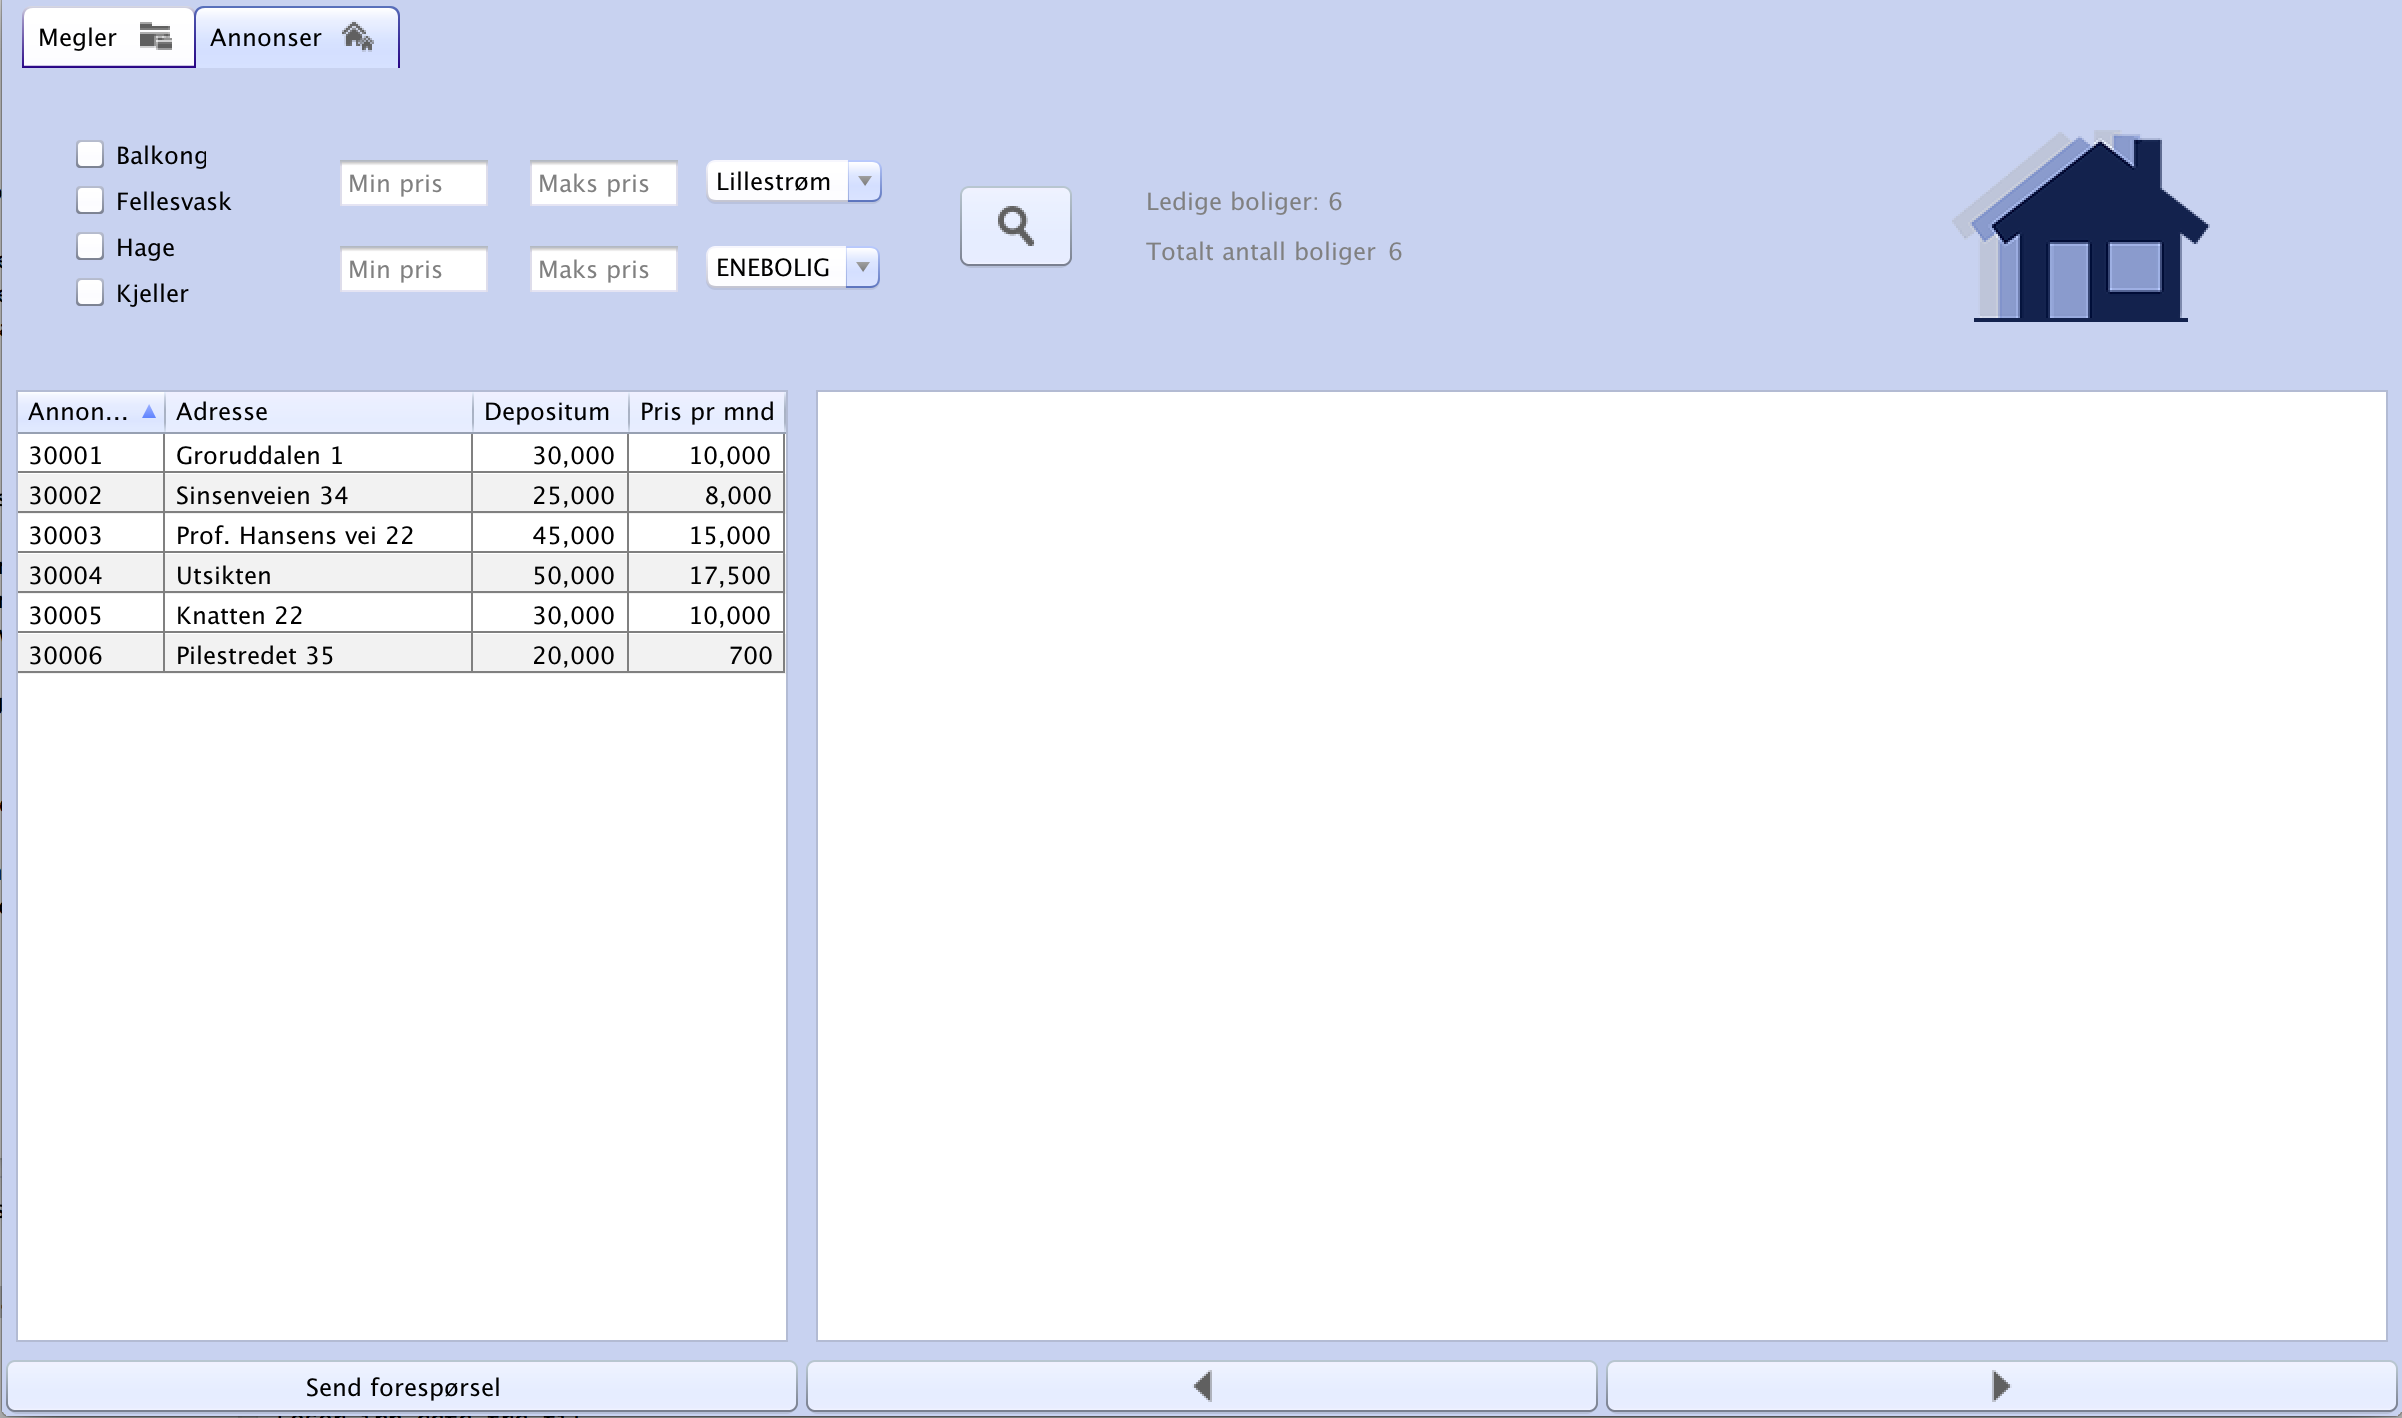
\includegraphics[width=\textwidth,height=\textheight,keepaspectratio]{./img/brukerveiledning/1.png}
 \caption{Boligsøkende.}
 \label{fig:bv:1}
\end{figure}




%//////////////////////////////////////////////

\section{Bolisøker}



\subsection{Filterpanel}

Dette er øverste del av programvinduet markert i rødt på figur \ref{fig:bv:2}. Her har en muligheten til å
legge inn ønskede søkekritierier, og søke blant tilgjengelige boliger ut ifra valgte kriterier.
En kan til enhver tid trykke på “Enter” knappen for å gjøre et søk ut ifra valgte kriterier, eller ved å
enkelt og greit trykke på søk-knappen.

Merk at tilgjengelige stedsnavn i dropdown menyen, vil kun vise stedsnavn for steder det er
registrert boliger for. Finner du ikke stedsnavnet ditt i denne listen, så er det heller ingen
tilgjengelige boliger i det aktuelle området.



\begin{figure}[h!]
 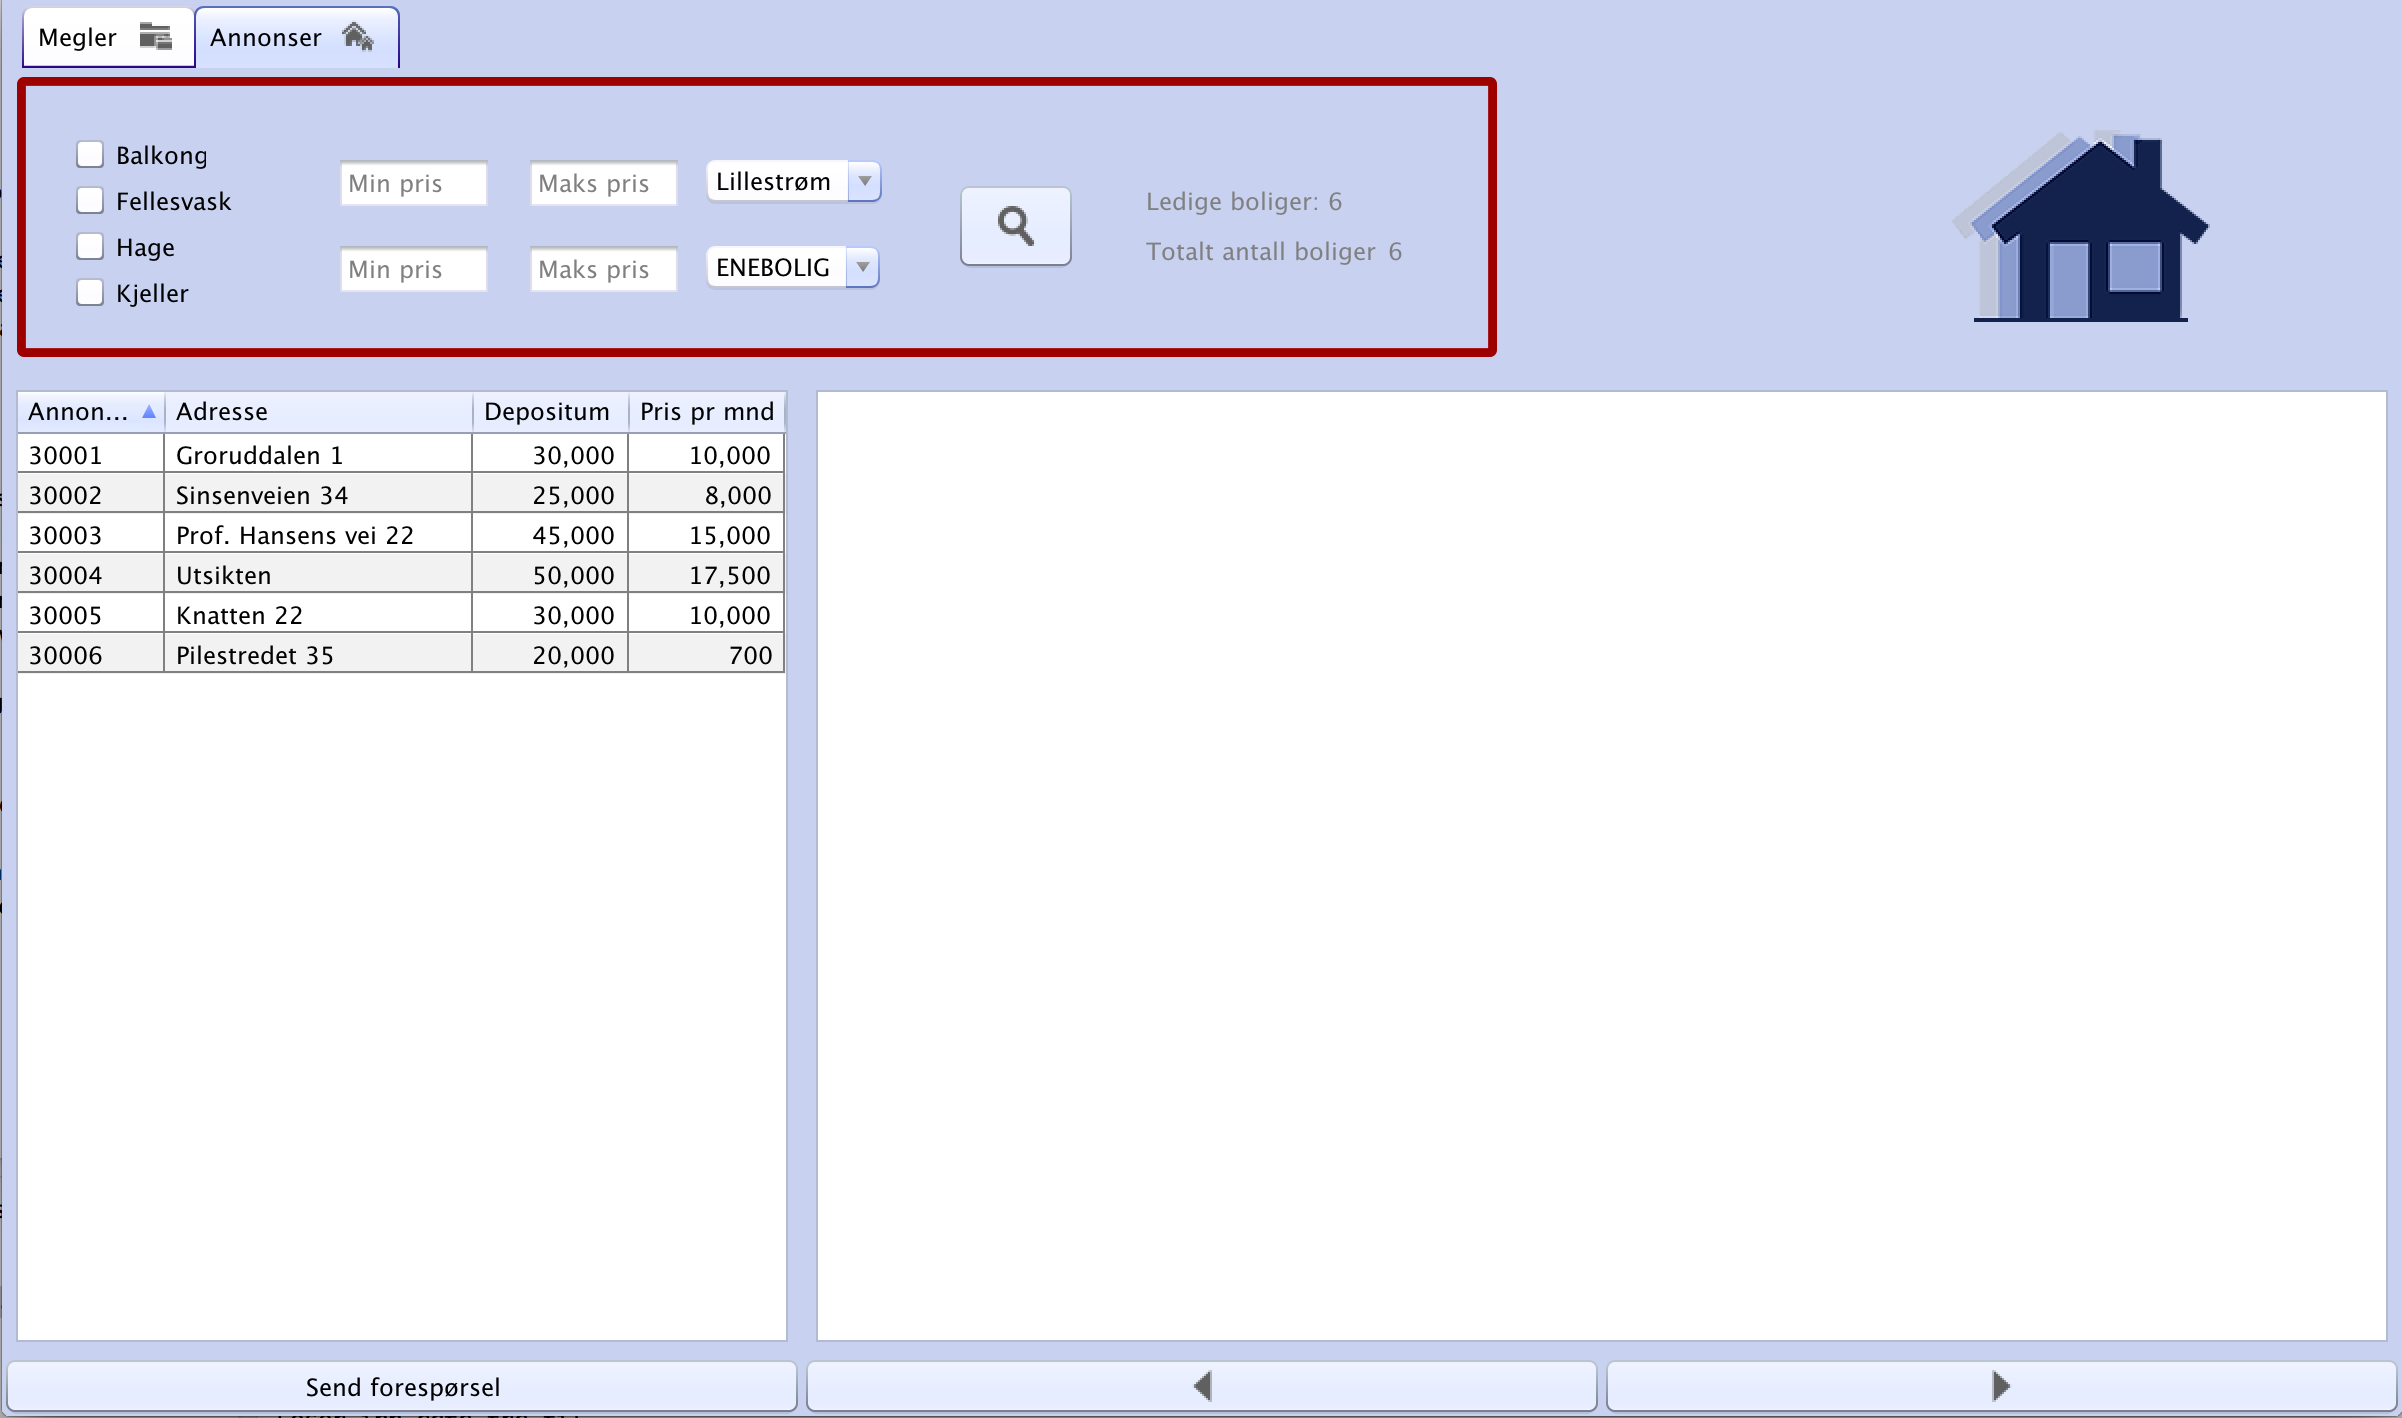
\includegraphics[width=\textwidth,height=\textheight,keepaspectratio]{./img/brukerveiledning/2.png}
 \caption{Filterpanel.}
 \label{fig:bv:2}
\end{figure}




\newpage
\subsection{Resultatabell}
Dette er venstre del av programvinduet, markert i rødt på figur \ref{fig:bv:3}.
Her vil resultater av et evnt. utført søk vises.

En har mulighet til å sortere på annonse ID, Adresse, Depositum, og pris per mnd øverst i
resultatvinduet. Du kan bla igjennom annonser ved å bruke pil opp, eller pil ned knappene, eller
alternativt bruke “fram og tilbake” knappene nederst til høyre i programvinduet.


\begin{figure}[h!]
 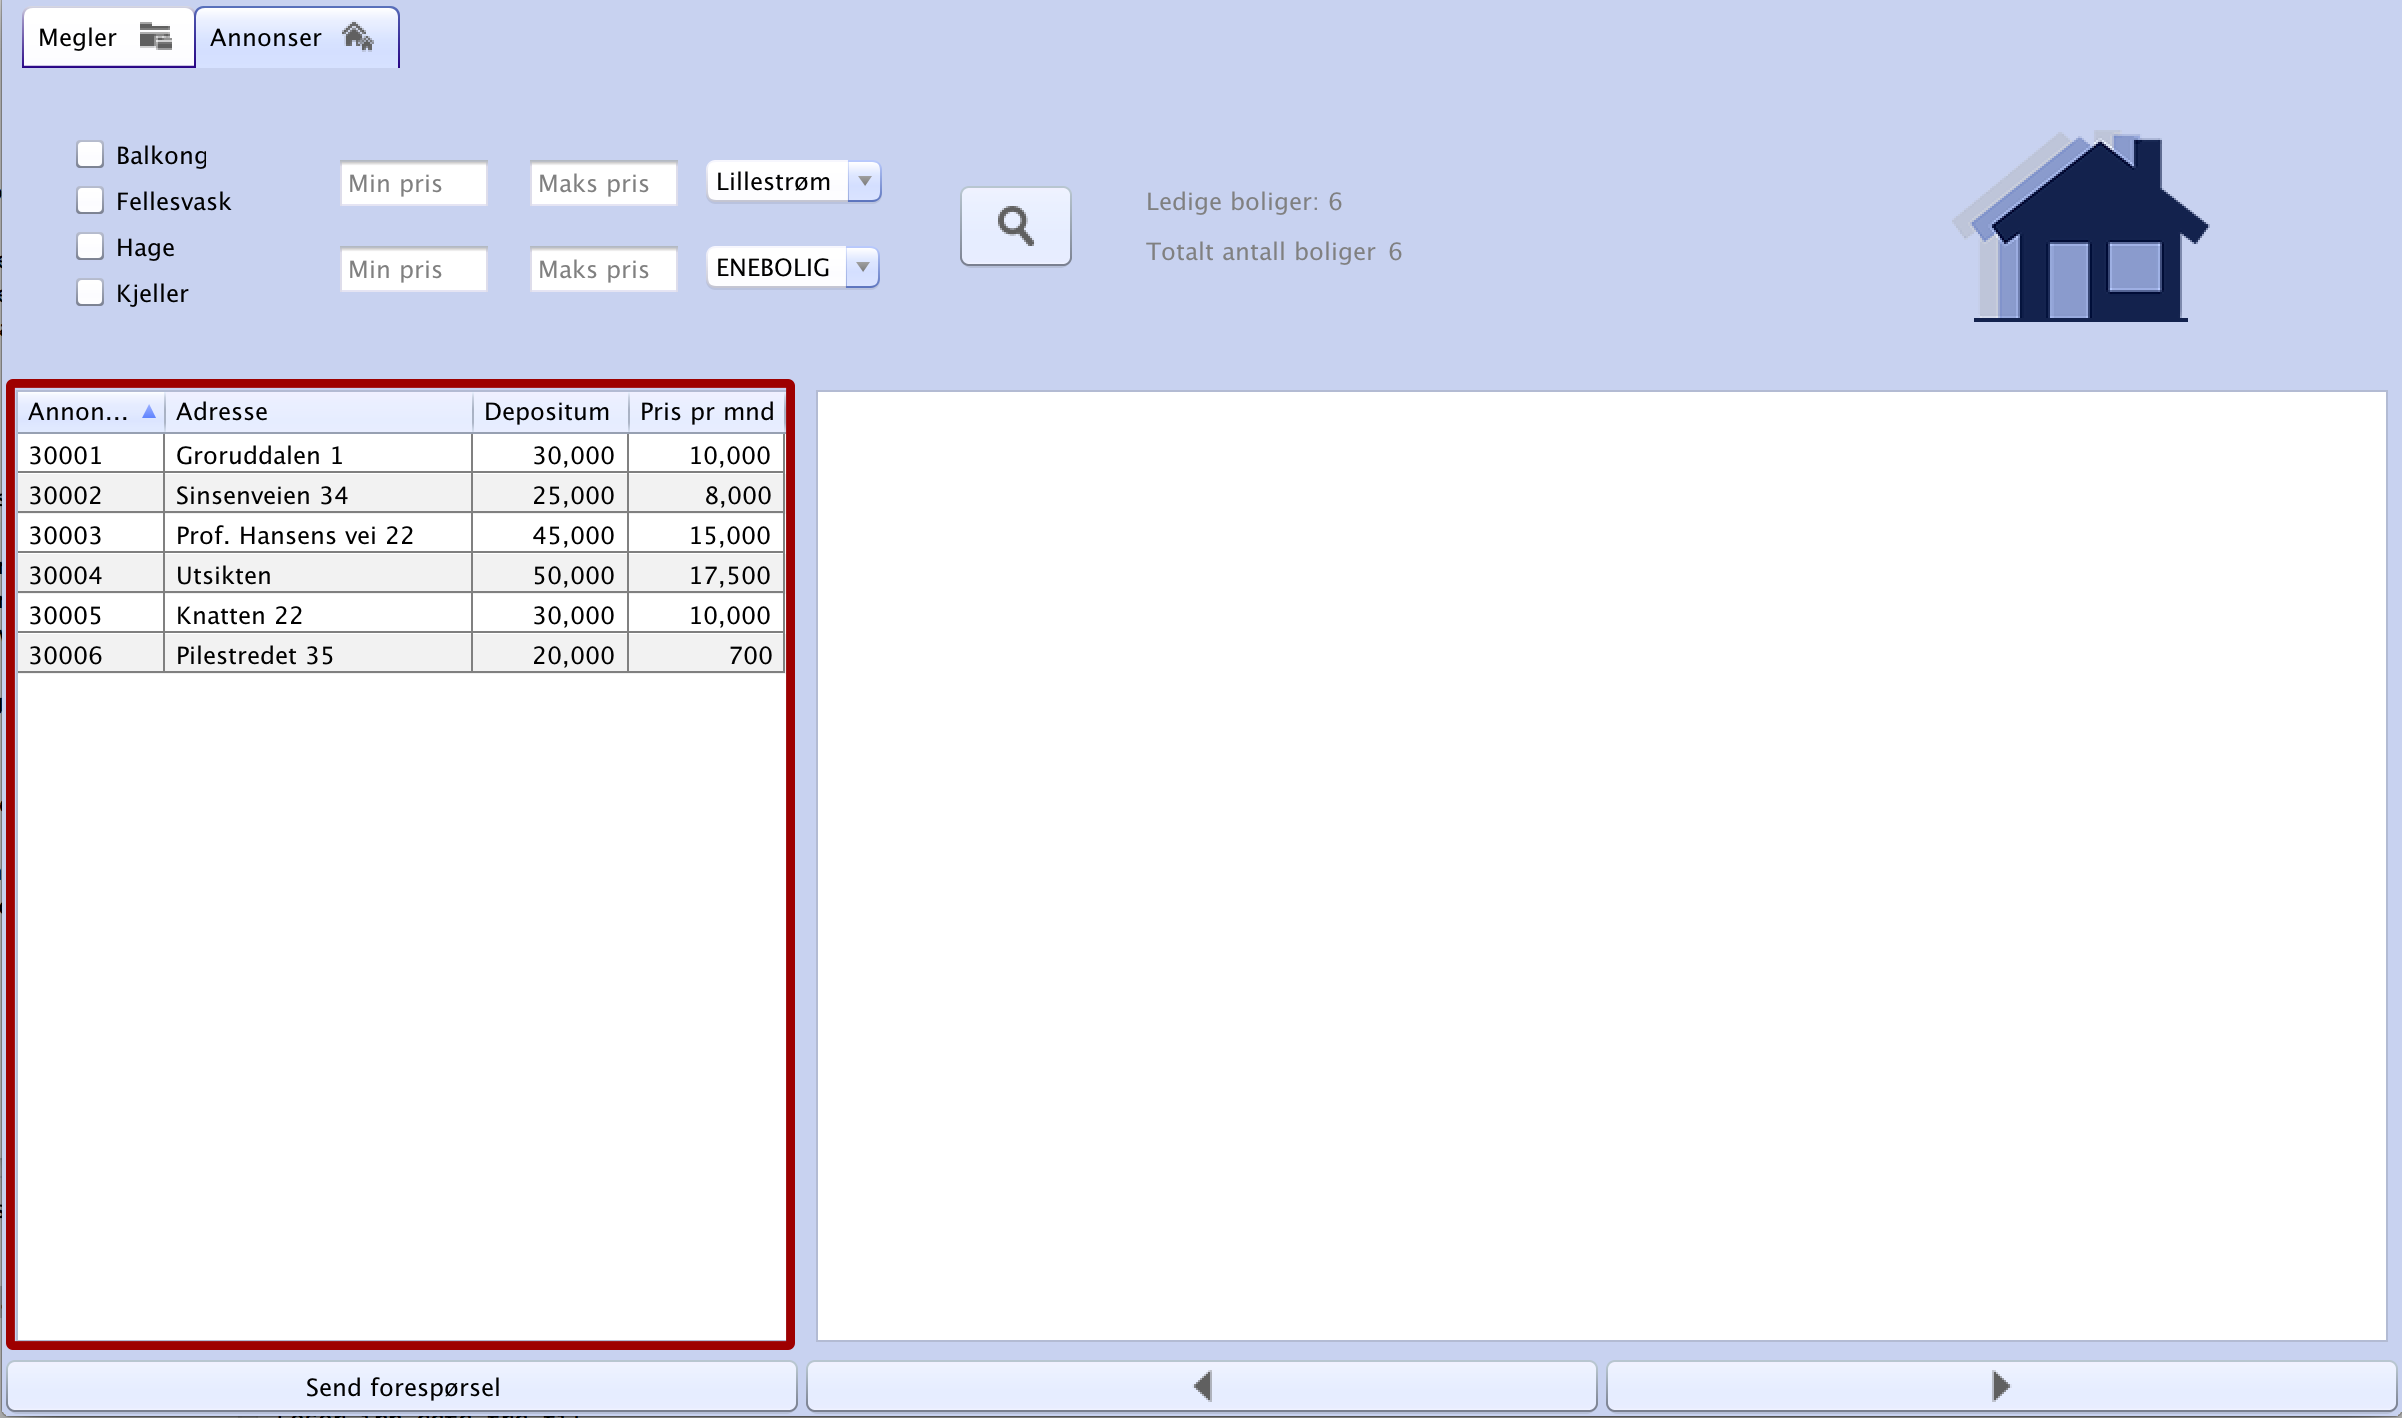
\includegraphics[width=\textwidth,height=\textheight,keepaspectratio]{./img/brukerveiledning/3.png}
 \caption{Resultattabell.}
 \label{fig:bv:3}
\end{figure}

Trykk på et treff i tabellen for å få fram flere detaljer om den valgte boligen i...




\newpage
\subsection{Visningspanel}

Her vil detaljer rundt valgt bolig (i resultattabellen) vises, markert i rødt på figur \ref{fig:bv:4}.


\begin{figure}[h!]
 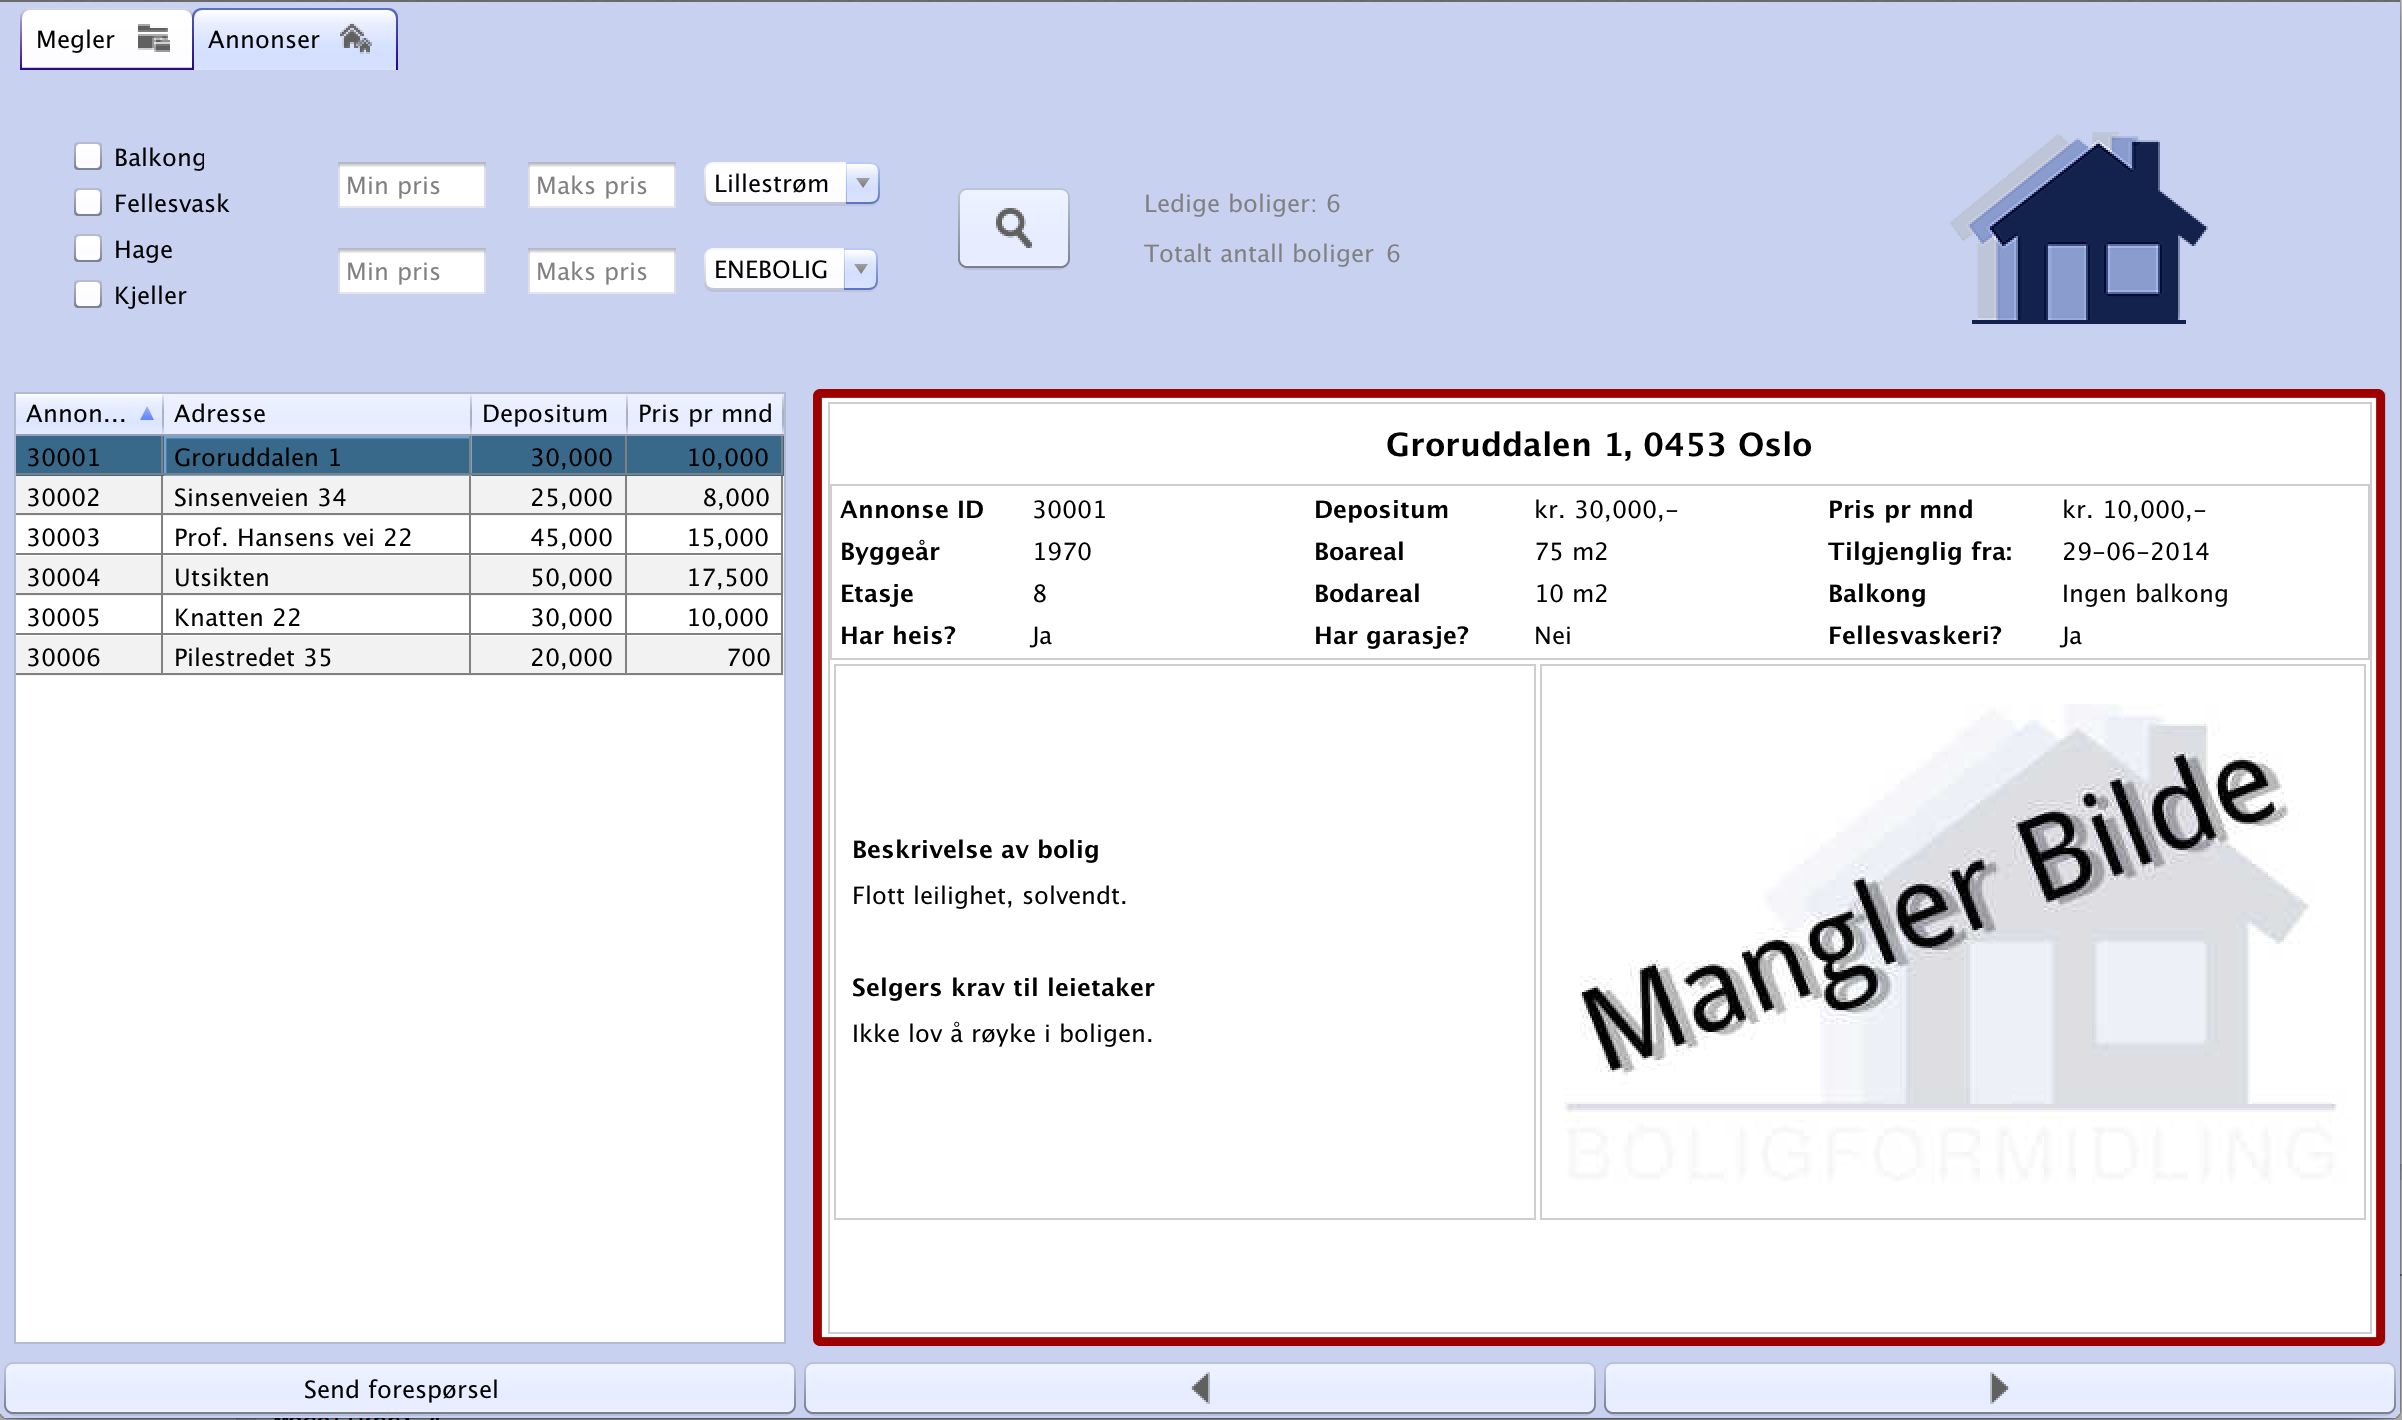
\includegraphics[width=\textwidth,height=\textheight,keepaspectratio]{./img/brukerveiledning/4.png}
 \caption{Visningspanel.}
 \label{fig:bv:4}
\end{figure}






\subsection{Forespørsel/søknad}
Trykk på “Send forespørsel” knappen nede i venstre hjørne av programmet (alternativt CTRL-F),
for sende inn din søknad på valgt bolig. Du vil da bli spurt om å akseptere evnt. spesielle vilkår
(figur \ref{fig:bv:5}) for den valgte boligen.

\begin{figure}[h!]
\center
 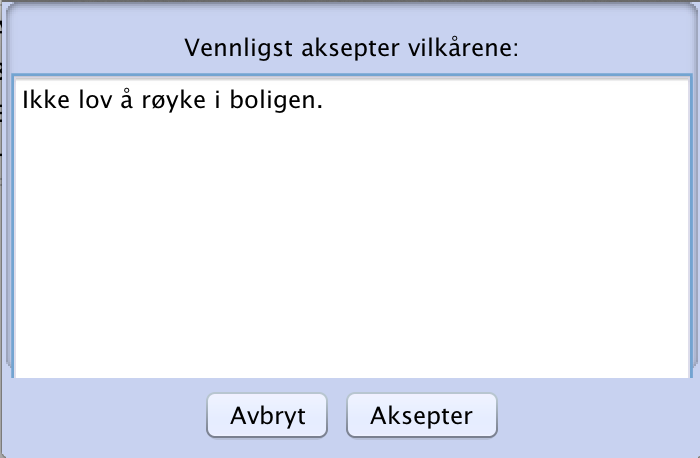
\includegraphics[scale=0.7]{./img/brukerveiledning/5.png}
 \caption{Forespørsel og krav fra utleier.}
 \label{fig:bv:5}
\end{figure}


Etter å evnt. ha akseptert vilkårene for den aktuelle boligen, så får en opp et nytt vindu med
mulighet for å skrive inn personalia mm. og sende inn søknad på boligen, som vist på figur \ref{fig:bv:6}.


\begin{figure}[h!]
\center
 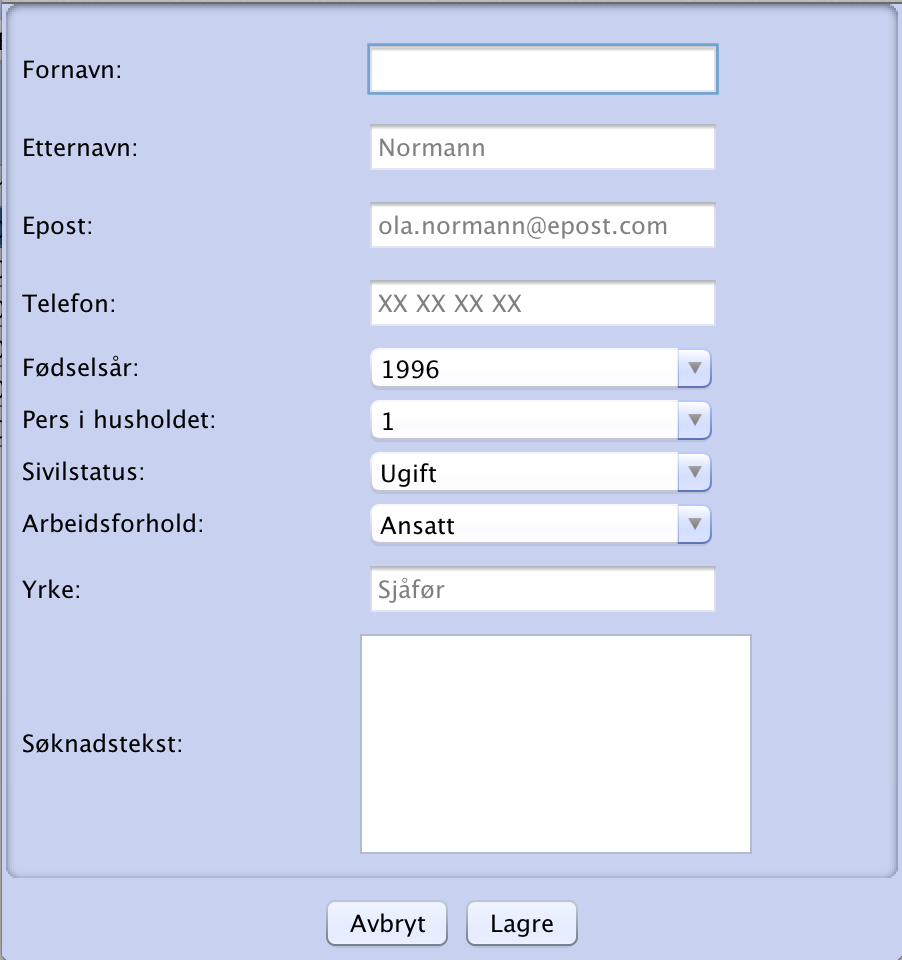
\includegraphics[scale=0.7]{./img/brukerveiledning/6.png}
 \caption{Registrering for leietaker.}
 \label{fig:bv:6}
\end{figure}





%////////////////////////////////////////////
\newpage
\section{Megler/administrasjon}

\subsection{Pålogging}

Ved å vege “Megler” arkfanen, så vil du først bli spurt om å logge deg inn som vist på figur \ref{fig:bv:7}.
Tast inn ditt brukernavn og passord, og trykk “Enter” for å logge inn, eller evnt. ved å trykke på “Ok”
knappen. Velger du “Avbryt” vil du komme tilbake til Annonse arkfanen igjen.

\begin{figure}[h!]
\center
 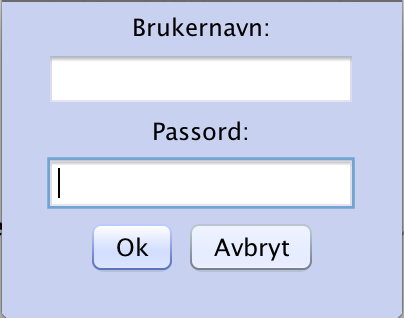
\includegraphics[scale=0.7]{./img/brukerveiledning/7.png}
 \caption{Pålogging for megler.}
 \label{fig:bv:7}
\end{figure}




\newpage
\subsection{Menyer}
øverste delen av programmet som vist på figur \ref{fig:bv:8}, så har du en knappe gruppe, som er ansvarlig
for administrasjon, mer spesifikt funksjonalitet for å opprette en ny utleier, ny bolig, ny annonse, og
en ny kontrakt.

Hvilke av disse funksjonene / knappene som er mulig å bruke, er avhengig av hva slags type
objekt du har valgt i i vinduet for søkeresultater. Mer spesifikt:

\begin{description}
\item[Ny Utleier] -
Kan brukes etter å ha søkt og valgt en annonse. \texttt{CTRL-U}
\item[Ny Bolig] -
Kan brukes etter å ha søkt og valgt blant utleiere. \texttt{CTRL-B}
\item[Ny Annonse] -
Kan brukes etter å ha søkt og valgt blant boliger. \texttt{CTRL-A}
\item[Ny Kontrakt] -
Kan brukes etter å ha søkt og valgt blant søknader. \texttt{CTRL-K}
\end{description}





\subsection{Søkepanel}
I øverste delen av programmet som vist på figur \ref{fig:bv:8}, så har du mulighet til å søke blant
ubehandlede boligsøknader, annonser, boliger, utleiere, leietakere, og eksisterende kontrakter.
Du må velge en kategori på venstre siden av søkefeltet for å kunne ta i bruk søkefunksjonaliteten,
ved hjelp av å trykke “Enter”, eller ved å enkelt og greit trykke på “søke-knappen”.


\begin{figure}[h!]
 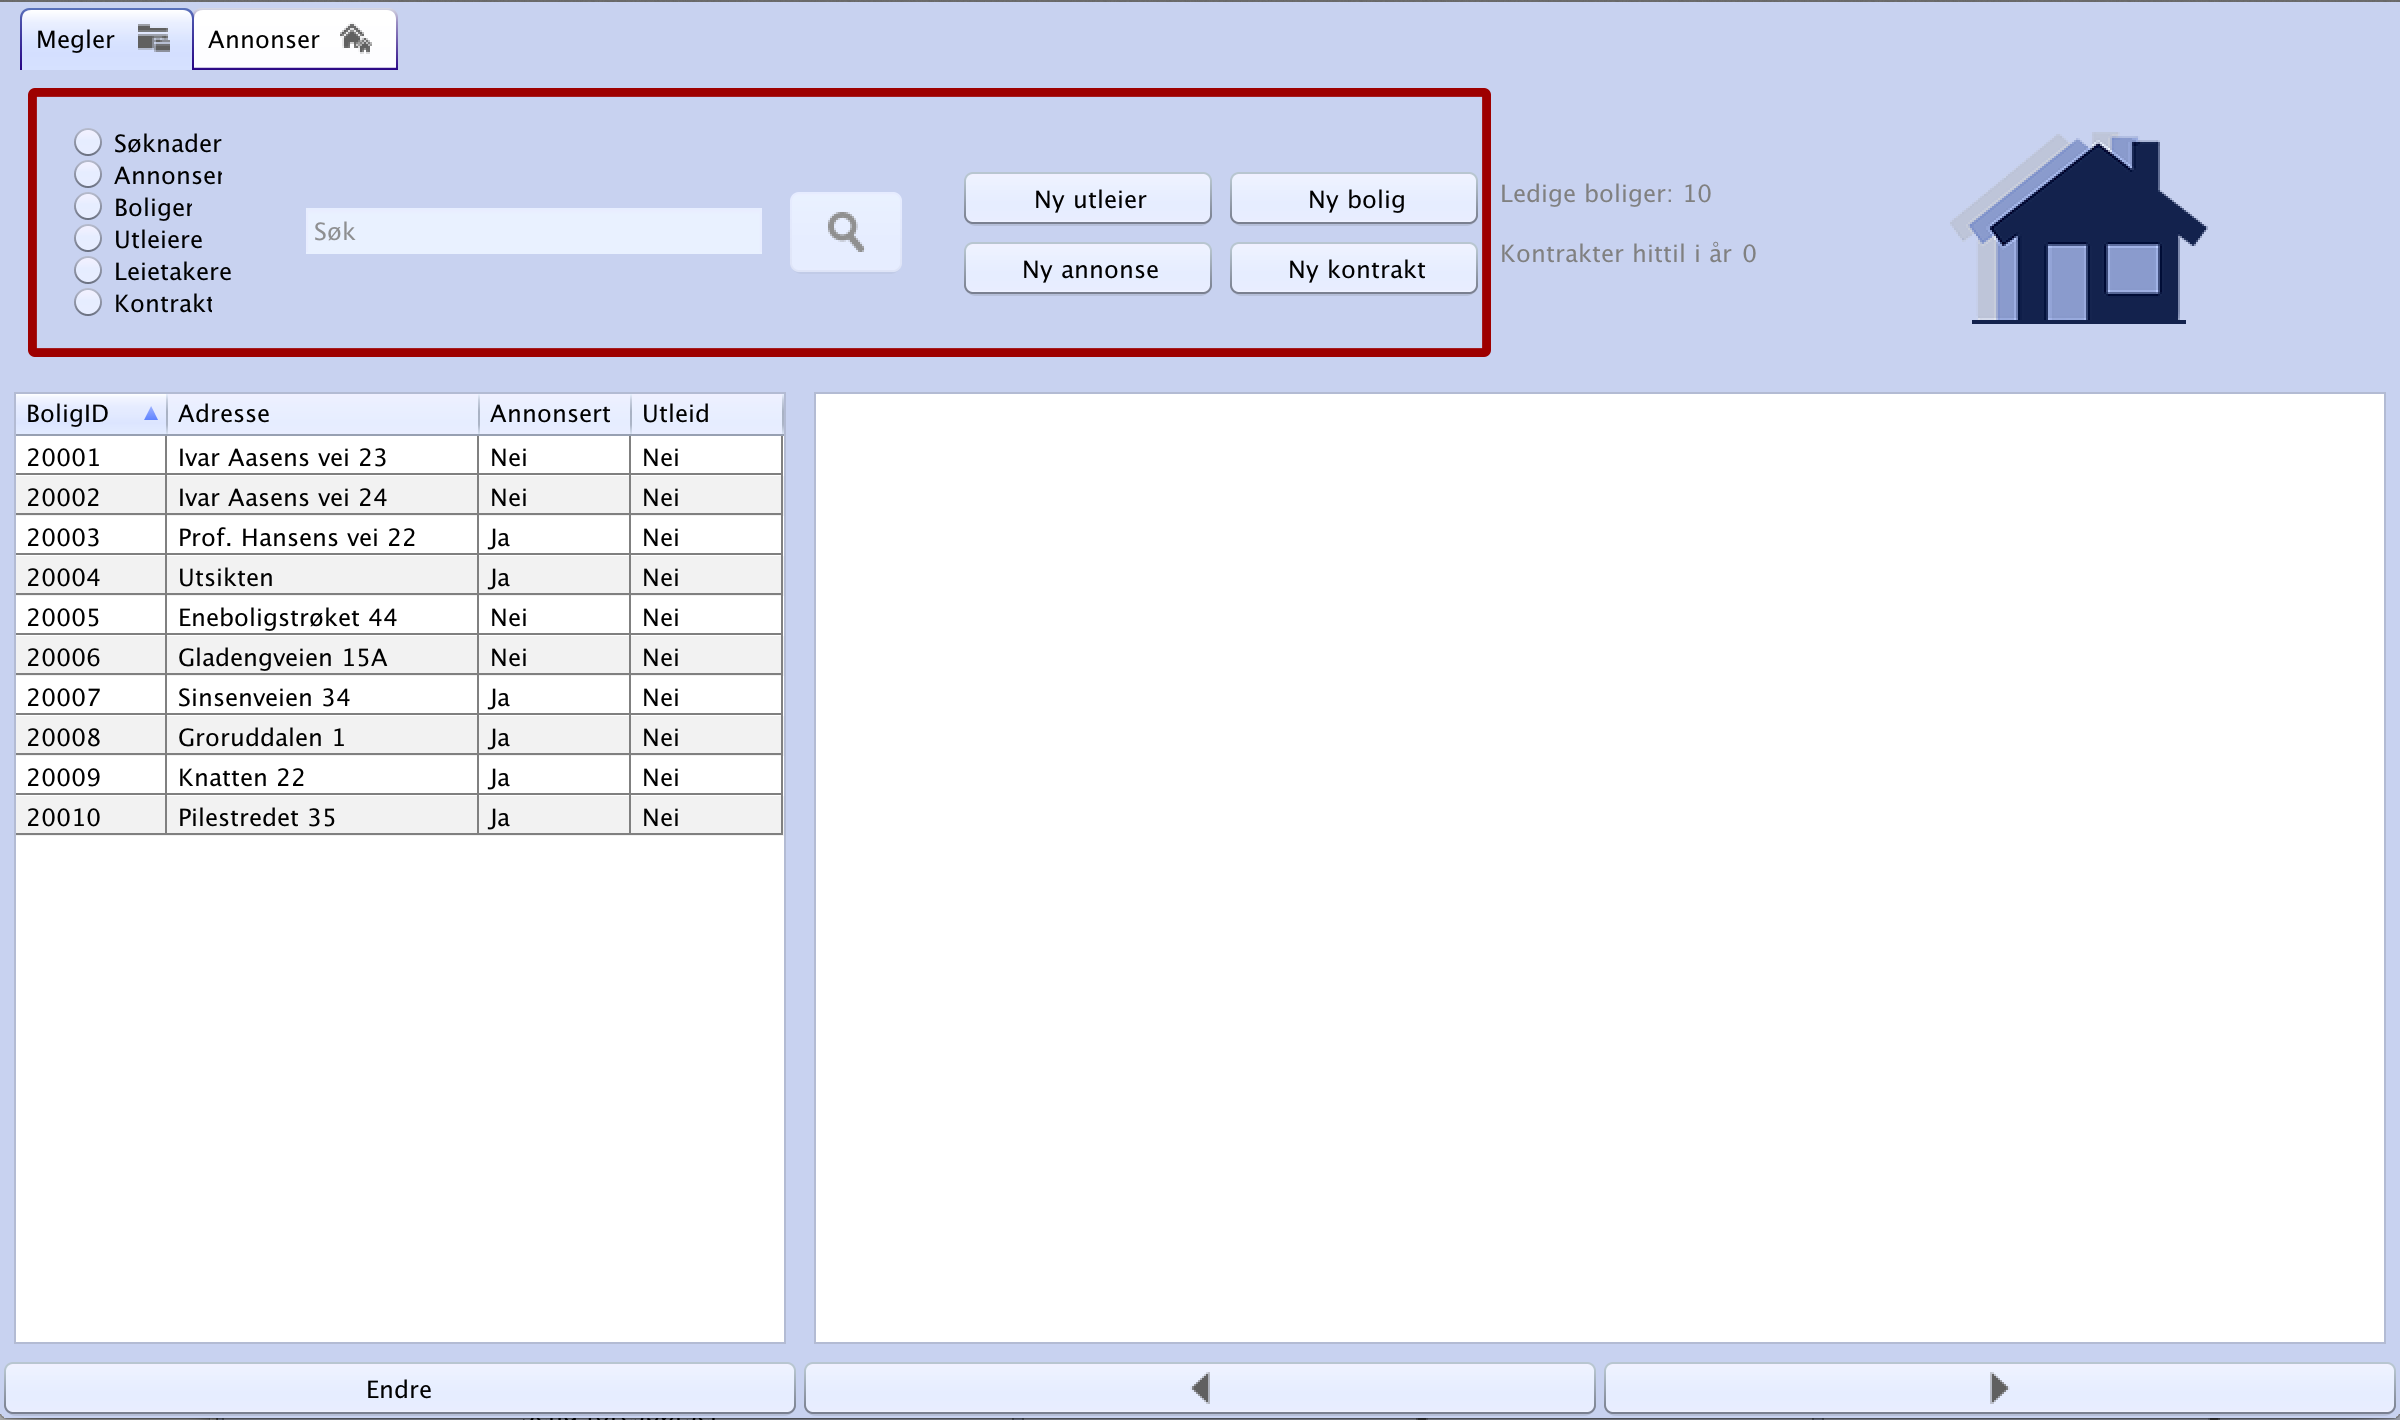
\includegraphics[width=\textwidth,height=\textheight,keepaspectratio]{./img/brukerveiledning/8.png}
 \caption{Søkepanel.}
 \label{fig:bv:8}
\end{figure}


\newpage
\subsection{Resultattabell}

Dette er venstre del av programvinduet, markert i rødt på figur \ref{fig:bv:9}. 
Her vil resultater av et evnt. utført søk vises. 

En har mulighet til å sortere på diverse kriterier øverst i resultatvinduet. Du kan bla igjennom
annonser ved å bruke pil opp, eller pil ned knappene, eller alternativt bruke “fram og tilbake”
knappene nederst til høyre i programvinduet.

\begin{figure}[h!]
 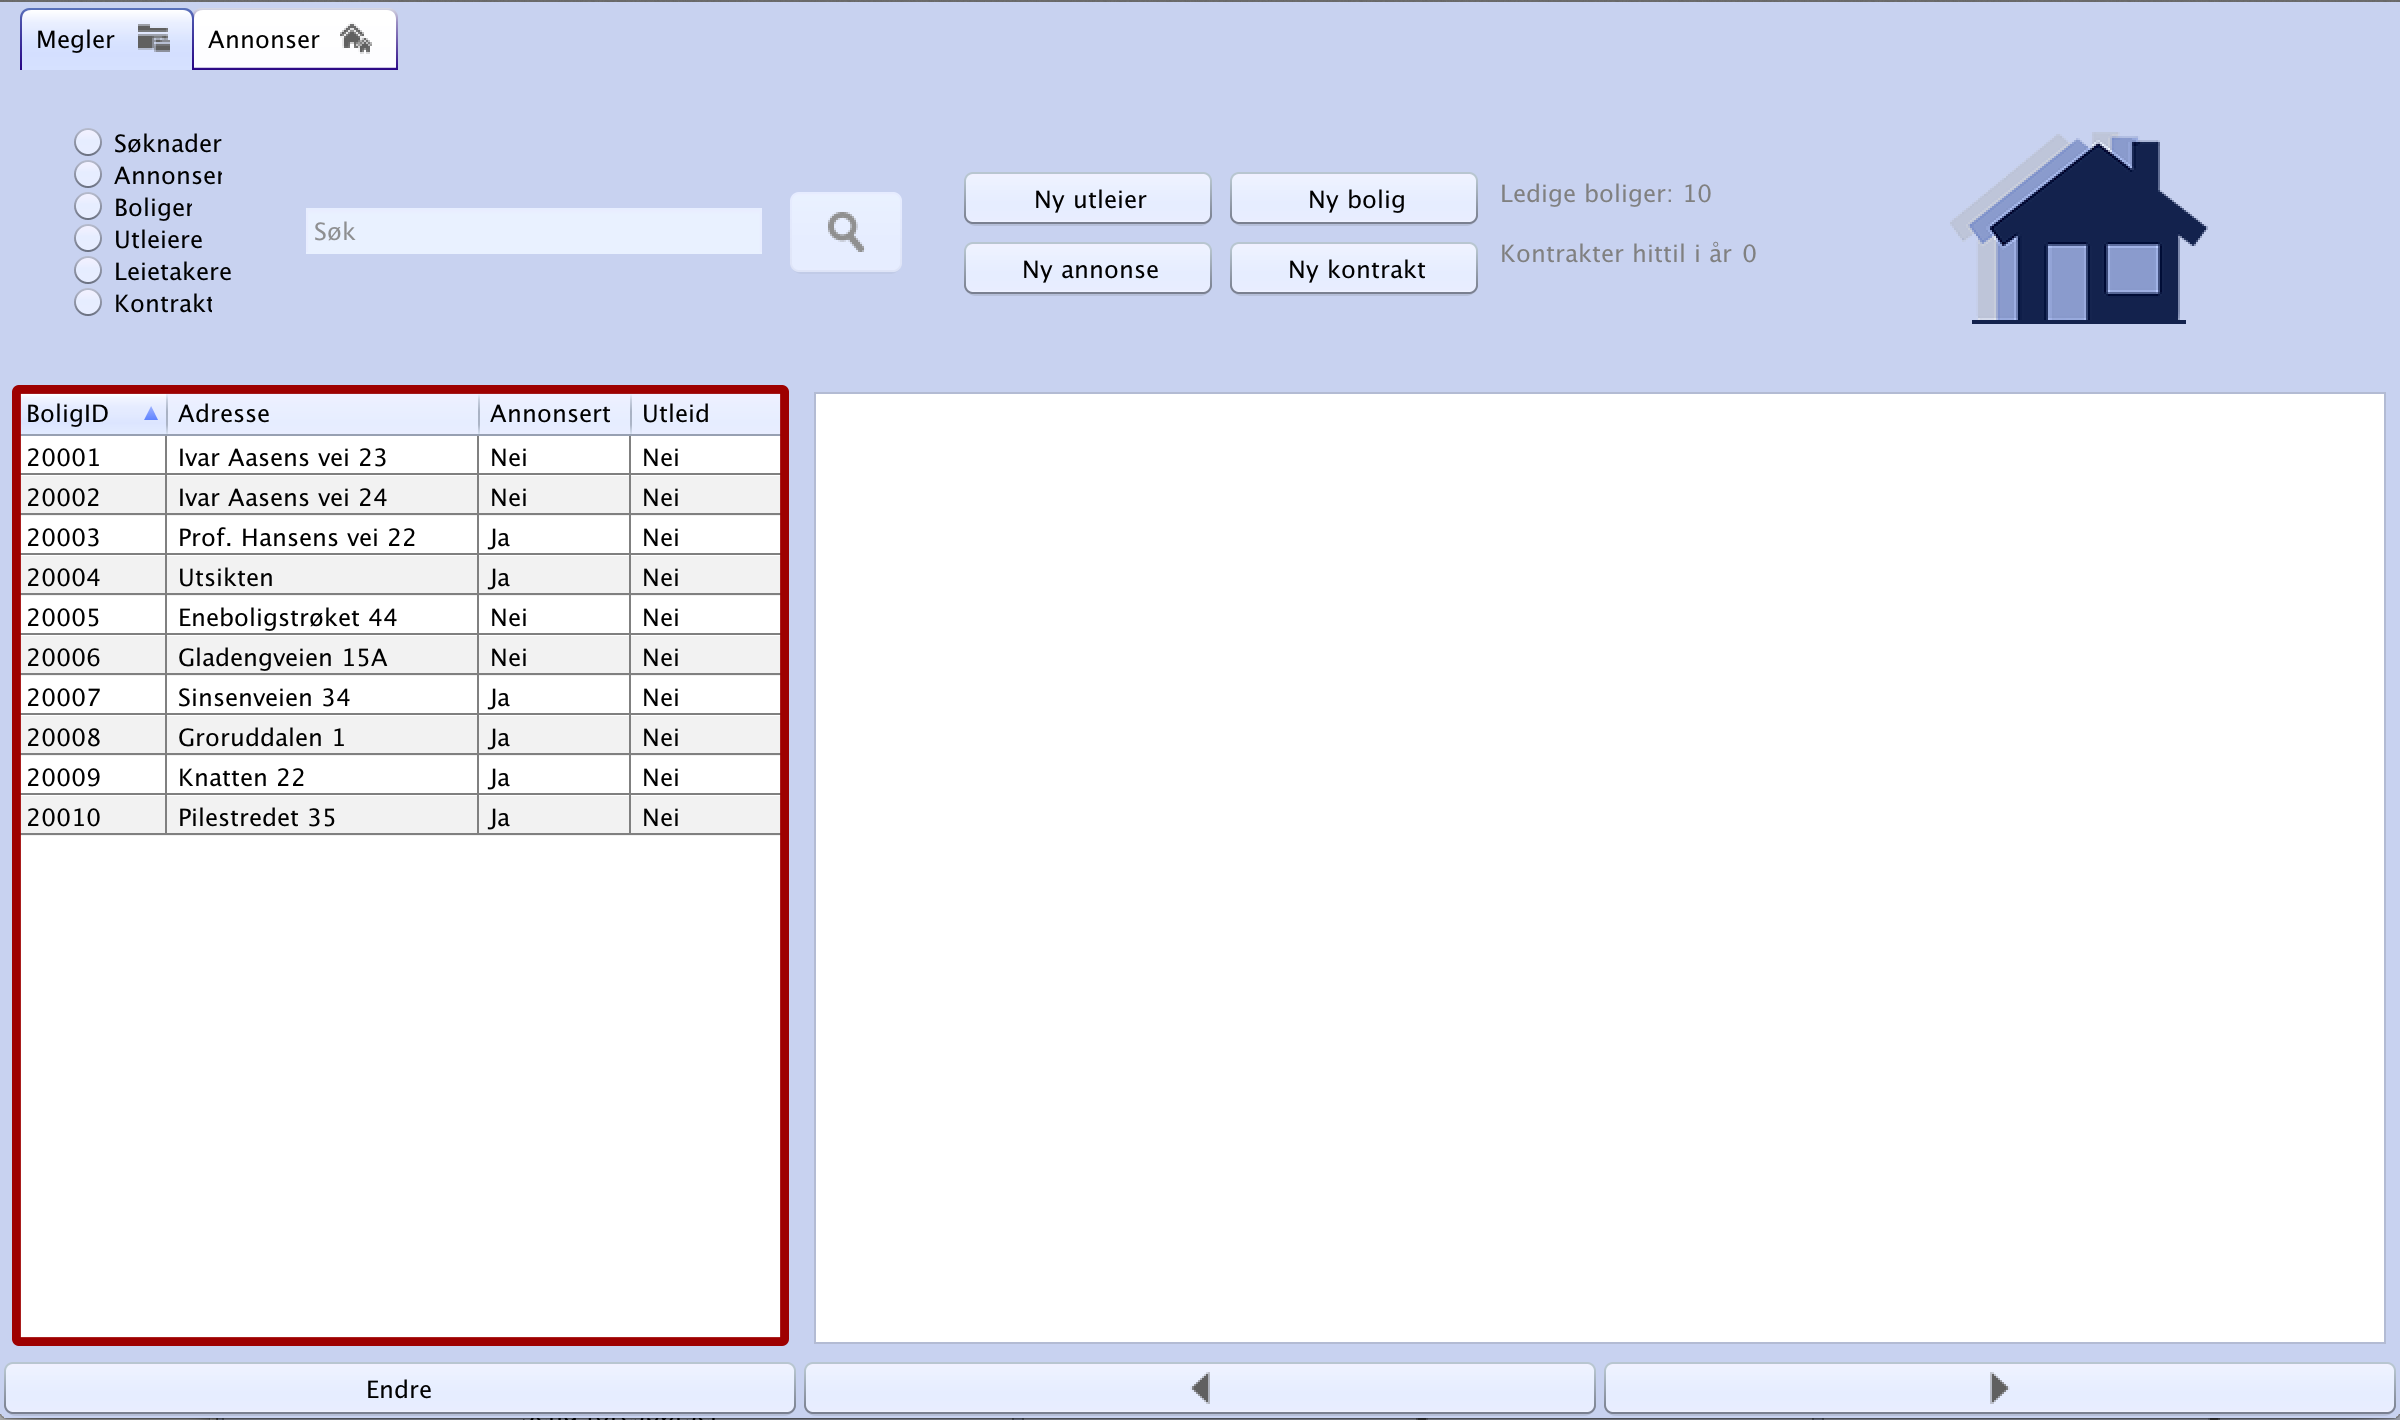
\includegraphics[width=\textwidth,height=\textheight,keepaspectratio]{./img/brukerveiledning/9.png}
 \caption{Resultattabell.}
 \label{fig:bv:9}
\end{figure}


\newpage
\subsection{Visningspanel}

Her vil detaljer rundt valgt objekt (i resultattabellen) vises, markert i rødt på figur \ref{fig:bv:10}.


\begin{figure}[h!]
 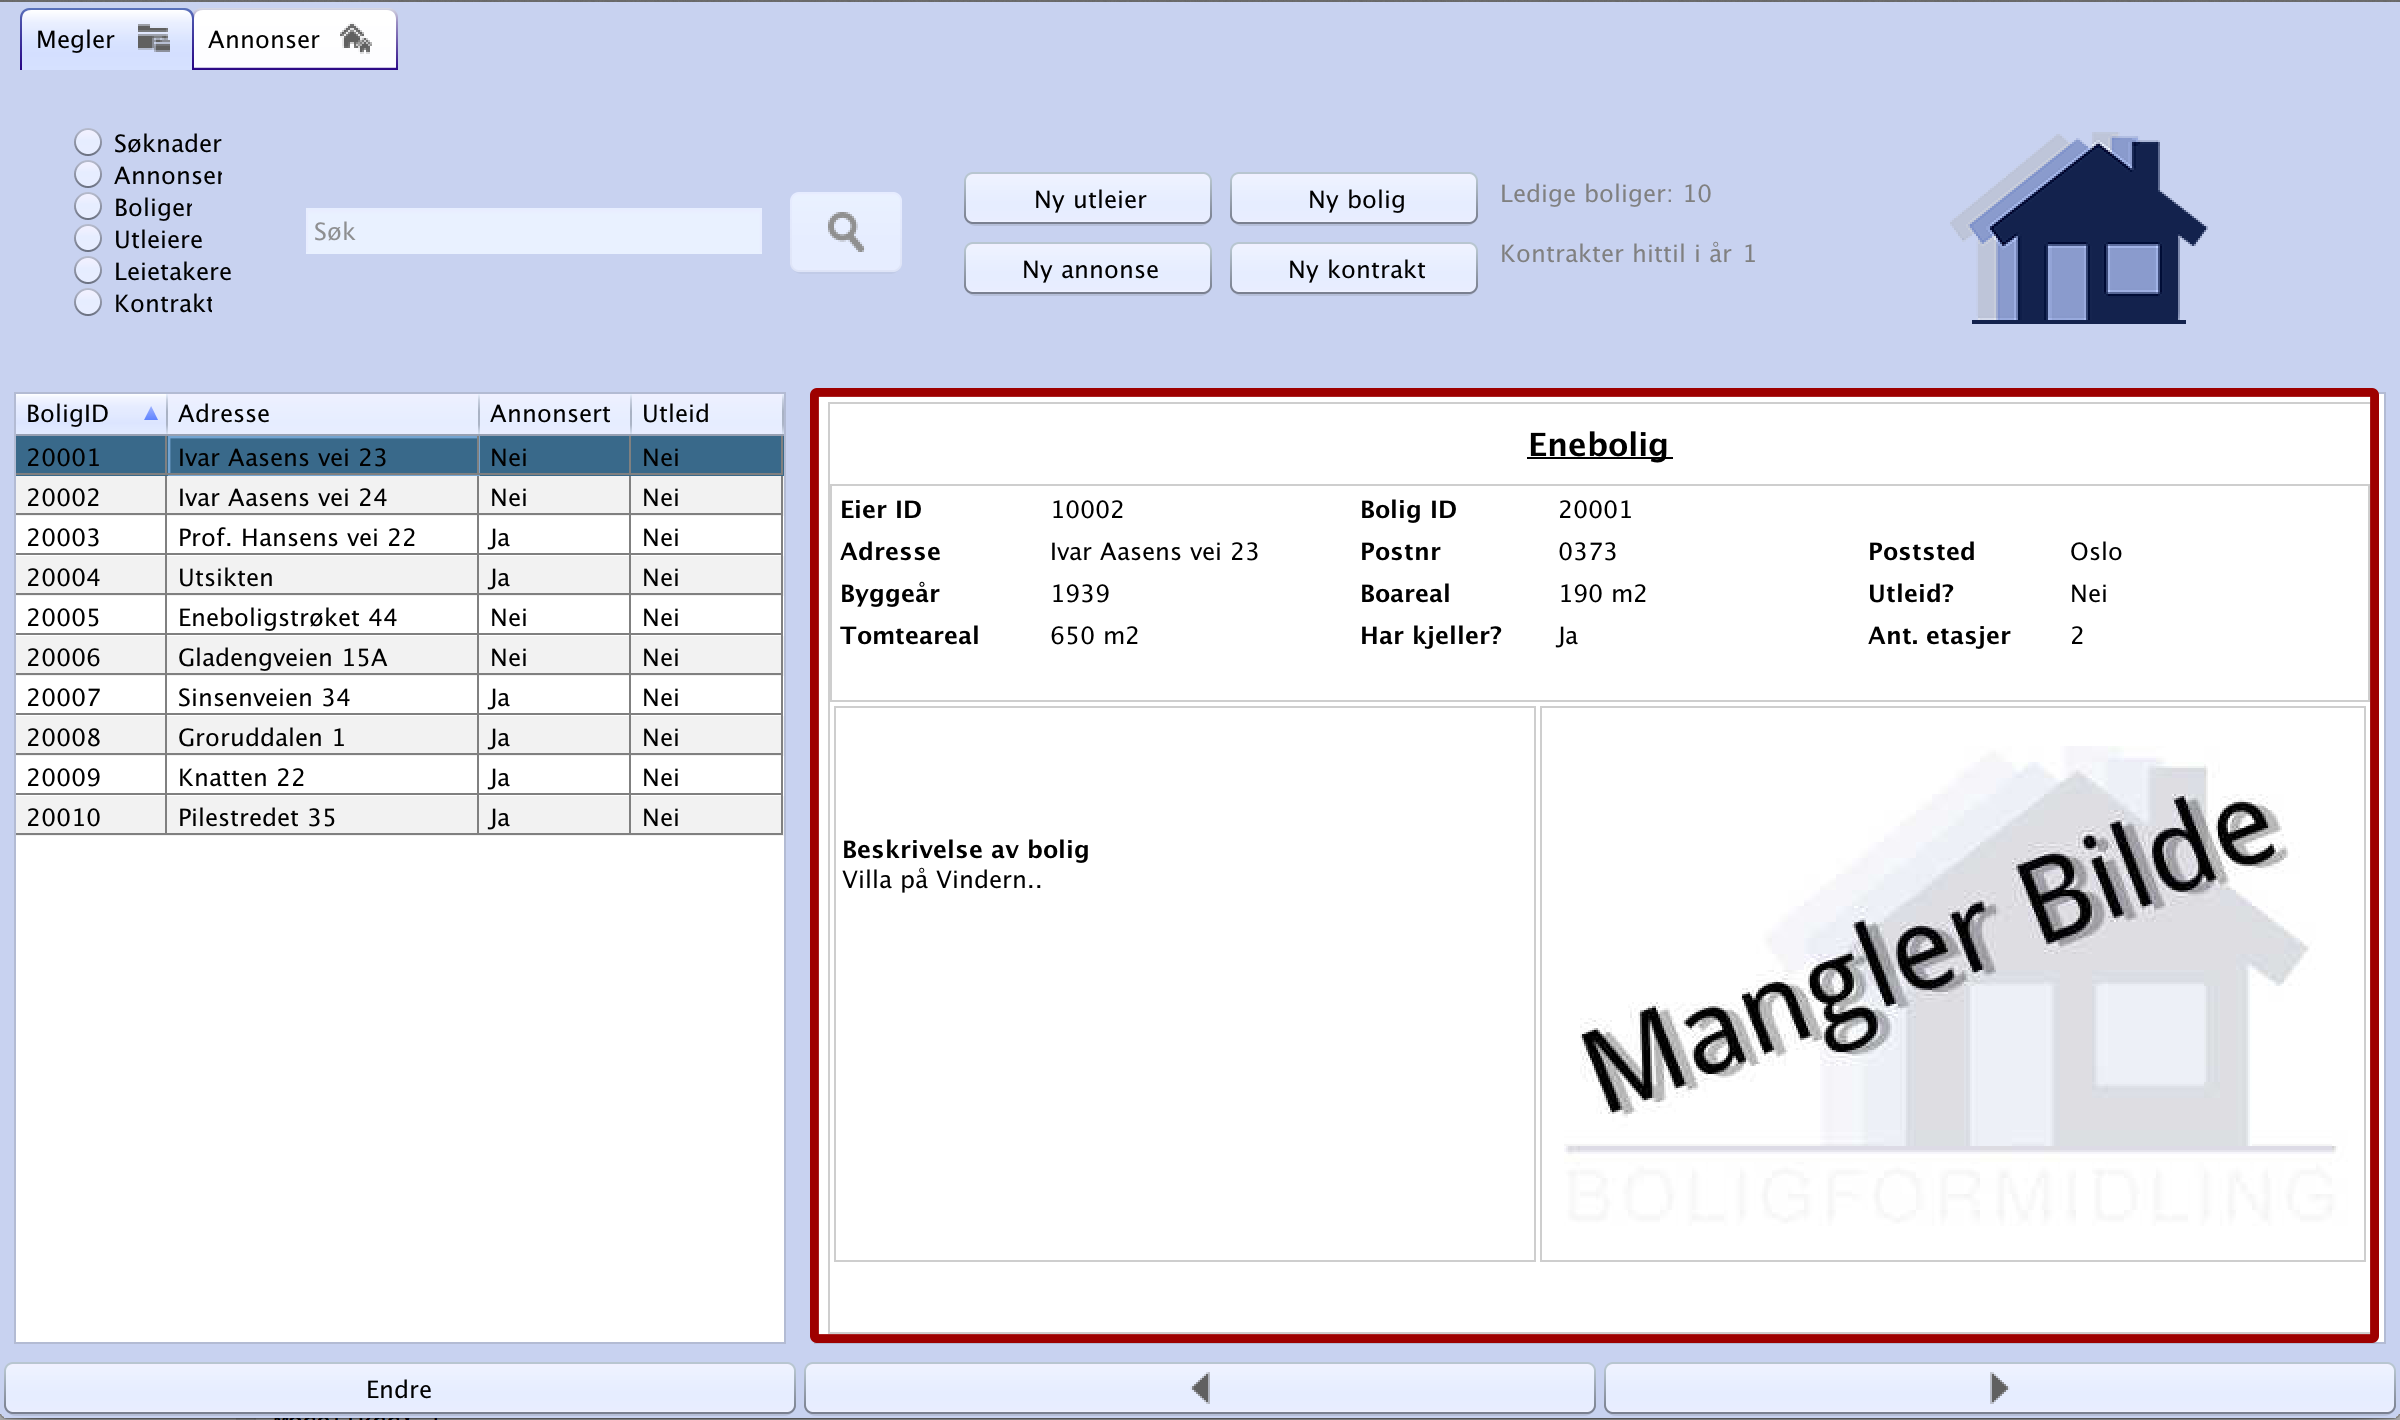
\includegraphics[width=\textwidth,height=\textheight,keepaspectratio]{./img/brukerveiledning/10.png}
 \caption{Visningspanel.}
 \label{fig:bv:10}
\end{figure}



\newpage
\subsection{Utleieradministrasjon}

Ved å søke blant utleiere, velge en person i listen, og trykke på “Endre” knappen nedest i venstre
hjørne av programvinduet, så har en mulighet til å gjøre endringer i informasjon lagret om
vedkommende, som vist på figur \ref{fig:bv:11}.

\begin{figure}[h!]
\center
 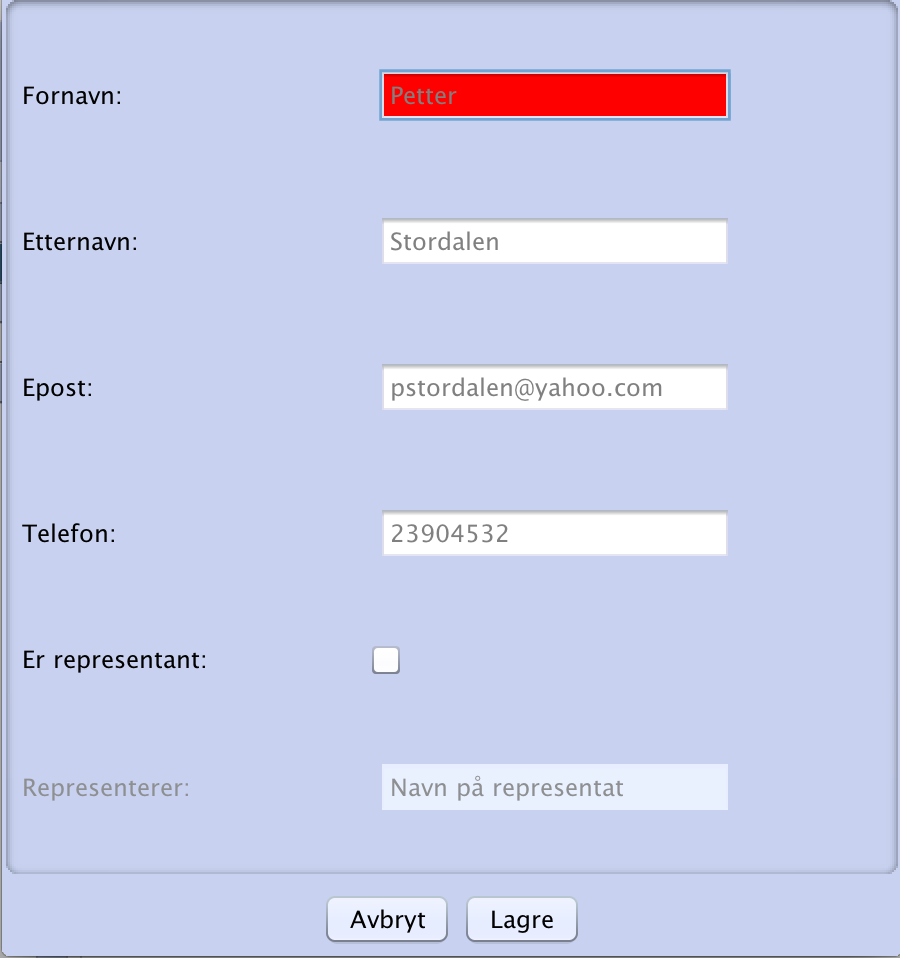
\includegraphics[scale=0.5]{./img/brukerveiledning/11.png}
 \caption{Utleieradministrasjon.}
 \label{fig:bv:11}
\end{figure}




\newpage
\subsection{Annonseadministrasjon}
ed å søke blant annonser, velge en annonse i listen, og trykke på “Endre” knappen nedest i venstre hjørne av programvinduet, så har en mulighet til å gjøre endringer i informasjon lagret om annonsen, som vist på figur \ref{fig:bv:12}.

\begin{figure}[h!]
 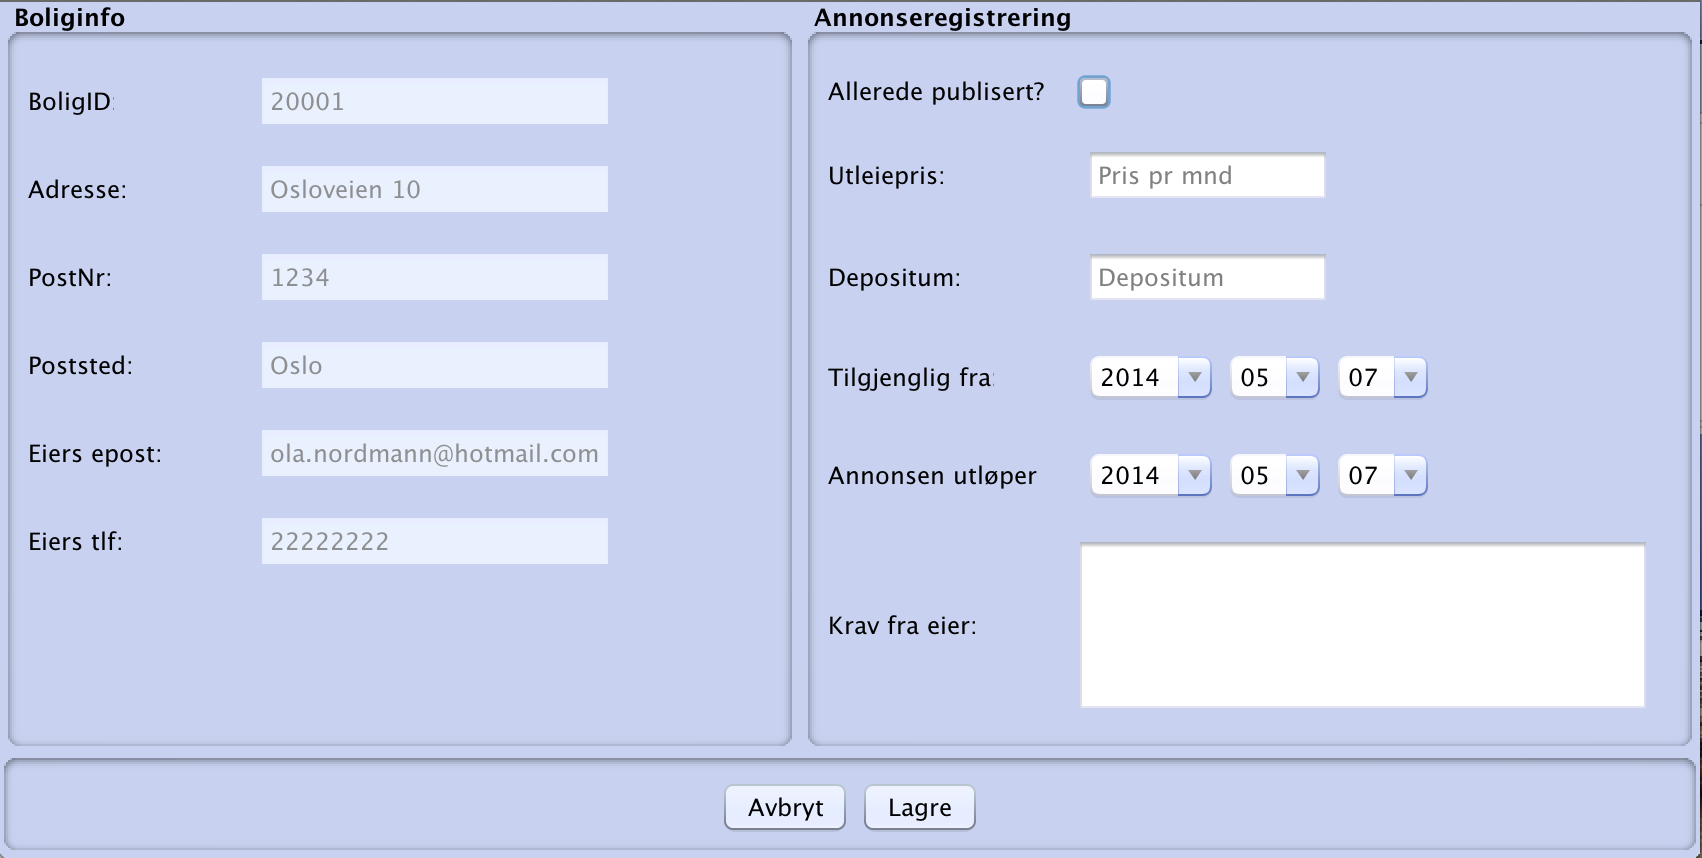
\includegraphics[width=\textwidth,height=\textheight,keepaspectratio]{./img/brukerveiledning/12.png}
 \caption{Annonseadministrasjon.}
 \label{fig:bv:12}
\end{figure}



\newpage
\subsection{Boligadministrasjon}
Ved å søke blant boliger, velge en bolig i listen, og trykke på “Endre” knappen nedest i venstre
hjørne av programvinduet, så har en mulighet til å gjøre endringer i informasjon lagret om boligen,
som vist på figur \ref{fig:bv:13}.

\begin{figure}[h!]
 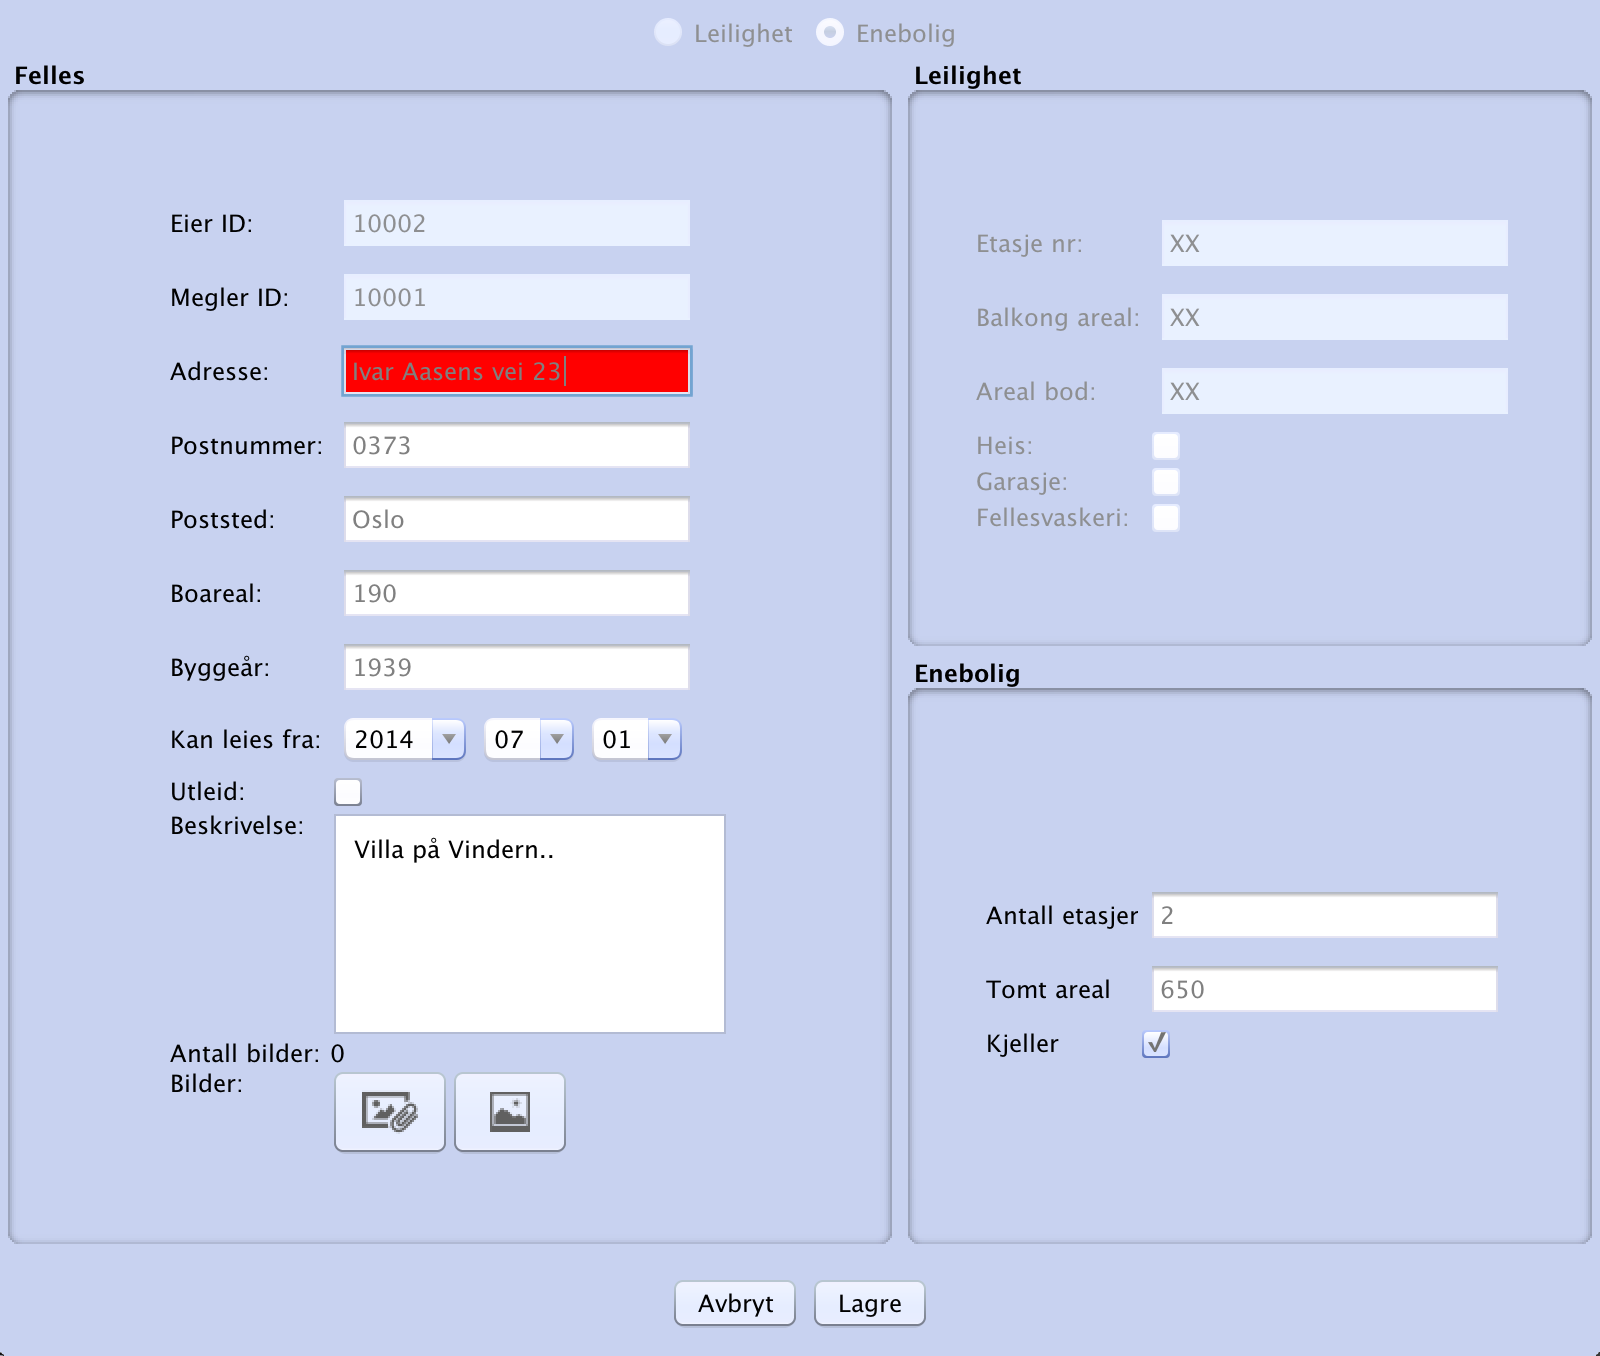
\includegraphics[width=\textwidth,height=\textheight,keepaspectratio]{./img/brukerveiledning/13.png}
 \caption{Boligadministrasjon.}
 \label{fig:bv:13}
\end{figure}


\newpage
\subsection{Kontraktadministrasjon}
Ved å søke etter innkommende søknader, velge en søknad i listen, og trykke på “Ny kontrakt”
knappen øverst i programvinduet, så har en mulighet til å godta, eller avslå den aktuelle søknaden.
Alternativt kan en høyreklikke på den aktuelle søknaden i listen, og velge godta/avslå derfra som
vist på figur \ref{fig:bv:14}. Er det flere søknader på en bolig, så vil de andre bli avslått ved en evnt.
godkjennelse av en søknad.

\begin{figure}[h!]
\center
 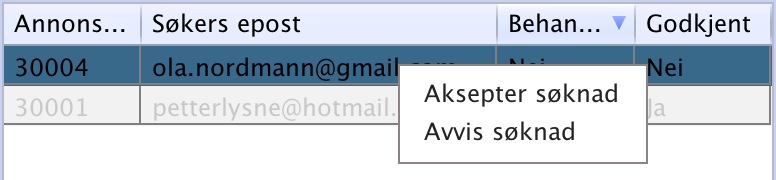
\includegraphics[scale=0.5]{./img/brukerveiledning/14.png}
 \caption{Kontraktadministrasjon.}
 \label{fig:bv:14}
\end{figure}



\subsection{Sletting}
Ved å høyreklikke på et objekt i resultatlisten, så har man mulighet til å slette det valgte objektet.
Alternativt kan “Delete” knappen brukes.

Det er imidlertid noen krav for å få slettet bestemte objekter. Mer spesifikt:

\begin{description}
\item[Slette utleiere] -
En kan ikke slette utleiere med eksisterende registrerte boliger. Boligene må i
såfall slettes først. Boliger som er utleid kan heller ikke slettes før de evnt. ikke lenger er utleid.
\end{description}



\subsection{Hurtigtaster/hotkeys}
For avanserte brukere, så kan hurtigtaster brukes for å oppnå høyere effektivitet, og kjappere
saksbehandling. Følgende hurtigtaster kan brukes:


\textbf{\underline{Generelt}}

\begin{description}
\item[\texttt{CTRL-Tab}] -
Skifter mellom annonse og megler arkfane / tab.
\item[\texttt{Enter/return}] -
Utfører et søk med gjeldende valgte søkekriterier.
\item[\texttt{Pil ned}] -
Blar nedover evnt. søketreff.
\item[\texttt{Pil opp}] -
Blar oppover evnt. søketreff.
\end{description}



\chapter{Testrapport}

\section{Begrensninger}

\subsection{Søk} \label{subsec:begrensinger:sok}
Søkeklassen for megler (avsnitt \ref{subsec:sok:megler}, side \pageref{subsec:sok:megler}) fungerer meget bra på de datamengder som programmet er testet på. På sikt burde det gjennomføres en rekke forbedringer i søket. Foreløpig itererer søket gjennom hele datasettet, selv om den skal returnere et tom søk. Søket er også alt for generelt, det medfører at søket resulterer alt for mange treff. For eksempel det er fullt mulig å søker med en enkel bokstav, hvis brukeren skriver "<a"> i søkefeltet blir alle objekter som inneholder den bokstaven i sine datafelt returnert. Eventuelle forbedringer som kan legges til kan være at brukeren kan spesifisere enkelte datafelt som man ønsker å søke i, i tillegg til ønsket register. For eksempel dersom man ønsker å søke i personregister på alle som har fornavn Ola, kan brukeren skrive søket med følgende "<syntaks">: \texttt{fornavn:Ola}. Slik søk vil da begrense søket til de spesifikke datafeltet.

\subsection{Generell brukeropplevelse}
Normalt sett vil et program ha mer funksjonalitet for sluttbruker enn det dette prosjektet tilbyr. Mangel av tid er hovedgrunnen til det, men også at vi ikke hadde et sterkere fokus på det spesifikke en sluttbruker ofte ønsker å få gjort helt fra starten.
Det var for så vidt et valg vi bevisst tok, om å fokusere på det tekniske, men skulle vi begynt på nytt er det klart at toppanel for både megler og annonse-visning ville sett litt annerledes ut. Programmet burde også kunne kjøres i "fullskjermvisning", noe vi valgte å ikke tillate da forskjellige skjermoppløsninger ville ødelegge layout for både tabell og visningsområde for objektene.

\section{Kjente feil \texttt{(Bugs)}}

\section{Forbedringer}



%Her kommer eksmpler som vi kan bruke nå man skal lage latex i rapporten
%\chapter{Kort bruksanvisning i \LaTeX{}}

Stortingets Tibetkomité består av enkeltrepresentanter med et spesielt sterkt 
engasjement for Tibet. Etter stortingsvalget høsten 2013 tok Venstres Ketil 
Kjenseth på seg en koordinerende rolle, og sendte i januar ut en mail til alle 
stortingsrepresentanter om hvem som kunne tenke seg å bidra.
Til tross for at Høyre åpner sitt landsmøte på Gardermoen fredag formiddag har 
fem stortingsrepresentanter fra regjeringspartiet funnet plass i programmet til 
å møte tibetaneren: Michael Tetzschner, Heidi Nordby Lunde, Erik Skutle, Anders 
B. Werp og Peter Chr. Frølich. Også Unge Høyre-leder Paul Joakim Sandøy er med 
og tar imot Dalai Lama.

\section{Kode}
Her kommer litt javakode for å teste ut hvorda det kommer til å se ut.

\begin{lstlisting}[title=Eksempelkode, caption=Koden teller til 1000, label=brakode]
class KnappeLytter implements ActionListener {

        @Override
        public void actionPerformed(ActionEvent e) {
            if (e.getSource().equals(vindu.getLagreButton())) {
                if(erNyregistrering){
                    registrerNyLeietaker();
                }
            } else if (e.getSource().equals(vindu.getAvbrytButton())) {
                vindu.dispose();
            }
        }

    }
\end{lstlisting}


\section{Kode fra fil}
Slik kan man legge inn kode direkte fra en java fil

\lstinputlisting[title=Tellerklasse, caption=Koden her gir NullPointerException, label=java:test1]{./kode/latex_bruksanvisning/1.java}



\section{Liste}
Her kommer eksepel på en liste\footnote{Her legger man til en fotnot hvis man ønsker å kommentere noe.}
\begin{itemize}
 \item Epple
 \item Pære
 \item Frosker
 \item Banan
\end{itemize}



\section{Figurer}
\subsection{Eksempel 2}
\begin{figure}[ht]
 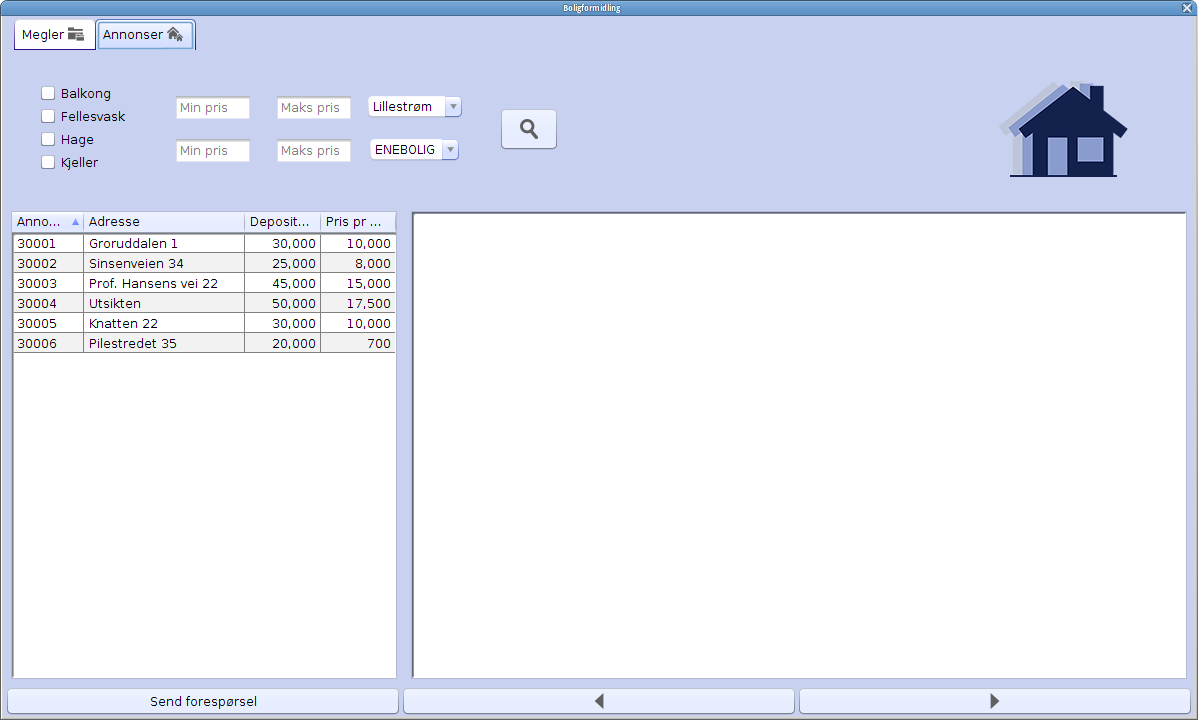
\includegraphics[width=\textwidth,height=\textheight,keepaspectratio]{./img/bruksanvisning/1.png}
 \caption{Dette er et eksempelbilde. Bilde blir automatisk numerert og lagt til i registeret.}
 %Her kommer en kabel for kryssreferering i teksten til figuren
 \label{fig:hovedvindu}
\end{figure}

\section{Referering}
Man må referer til alle figurer og kodeeksempel, som regel skal det ikke finnes en figur eller kodeeksempel dersom man ikke refererer til det i teksten. For at man skal kunne referer til noe så må man ha \textit{label} tag. For eksempel kan man nå referer til bilde gjennom følgende \ref{fig:hovedvindu}. \\
Man kan også ta en referanse til code gjennom \ref{java:test1}



%Appendix for vedlegg og andre ting som ikke direkte passer inn i resten av rapporten
\appendix

\chapter{Diagram} \label{appendix:diagram}

% IKKE SLETT VIL HA DENNE SOM EKSEMPEL
%\begin{figure}[ht]
% 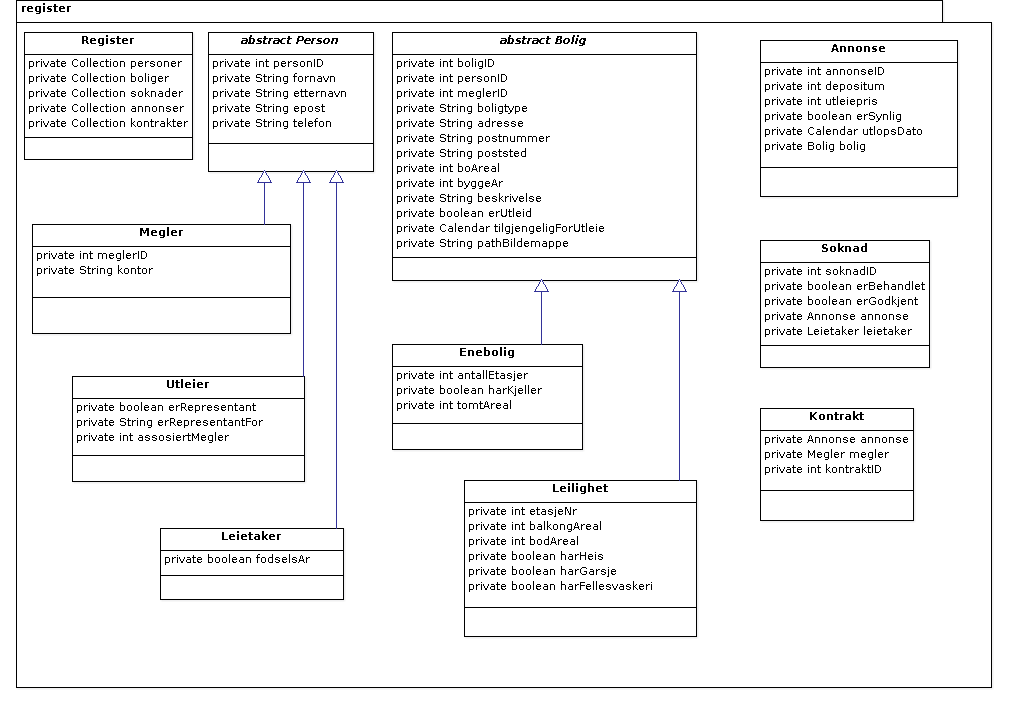
\includegraphics[angle=90 ,width=\textwidth,height=\textheight,keepaspectratio]{./img/appendix/diagram/klassestruktur_uml.png}
% \caption{Innledende UML diagram. brukt for generering av grunnleggende klasser.}
% %Her kommer en kabel for kryssreferering i teksten til figuren
% \label{fig:uml_diag}
%\end{figure}

\begin{figure}[ht]
\begin{center}
 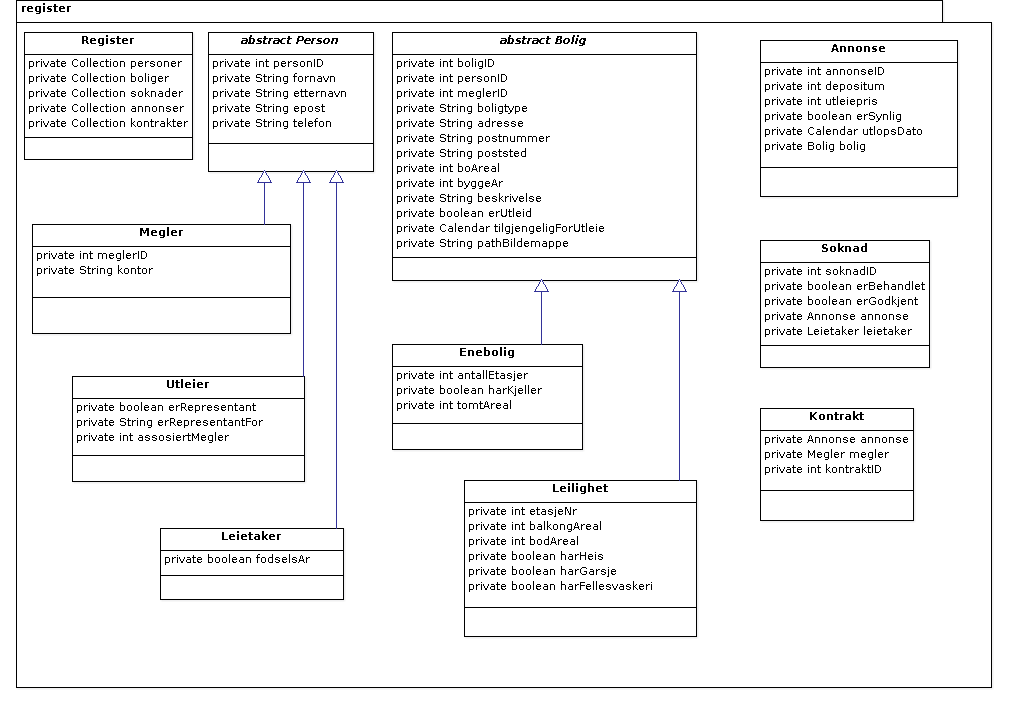
\includegraphics[angle=90, height=21cm]{./img/appendix/diagram/klassestruktur_uml.png}
 \caption{Innledende UML diagram. brukt for generering av grunnleggende klasser.}
 %Her kommer en kabel for kryssreferering i teksten til figuren
 \label{fig:uml_diag}
 \end{center}
\end{figure}


\begin{figure}[ht]
 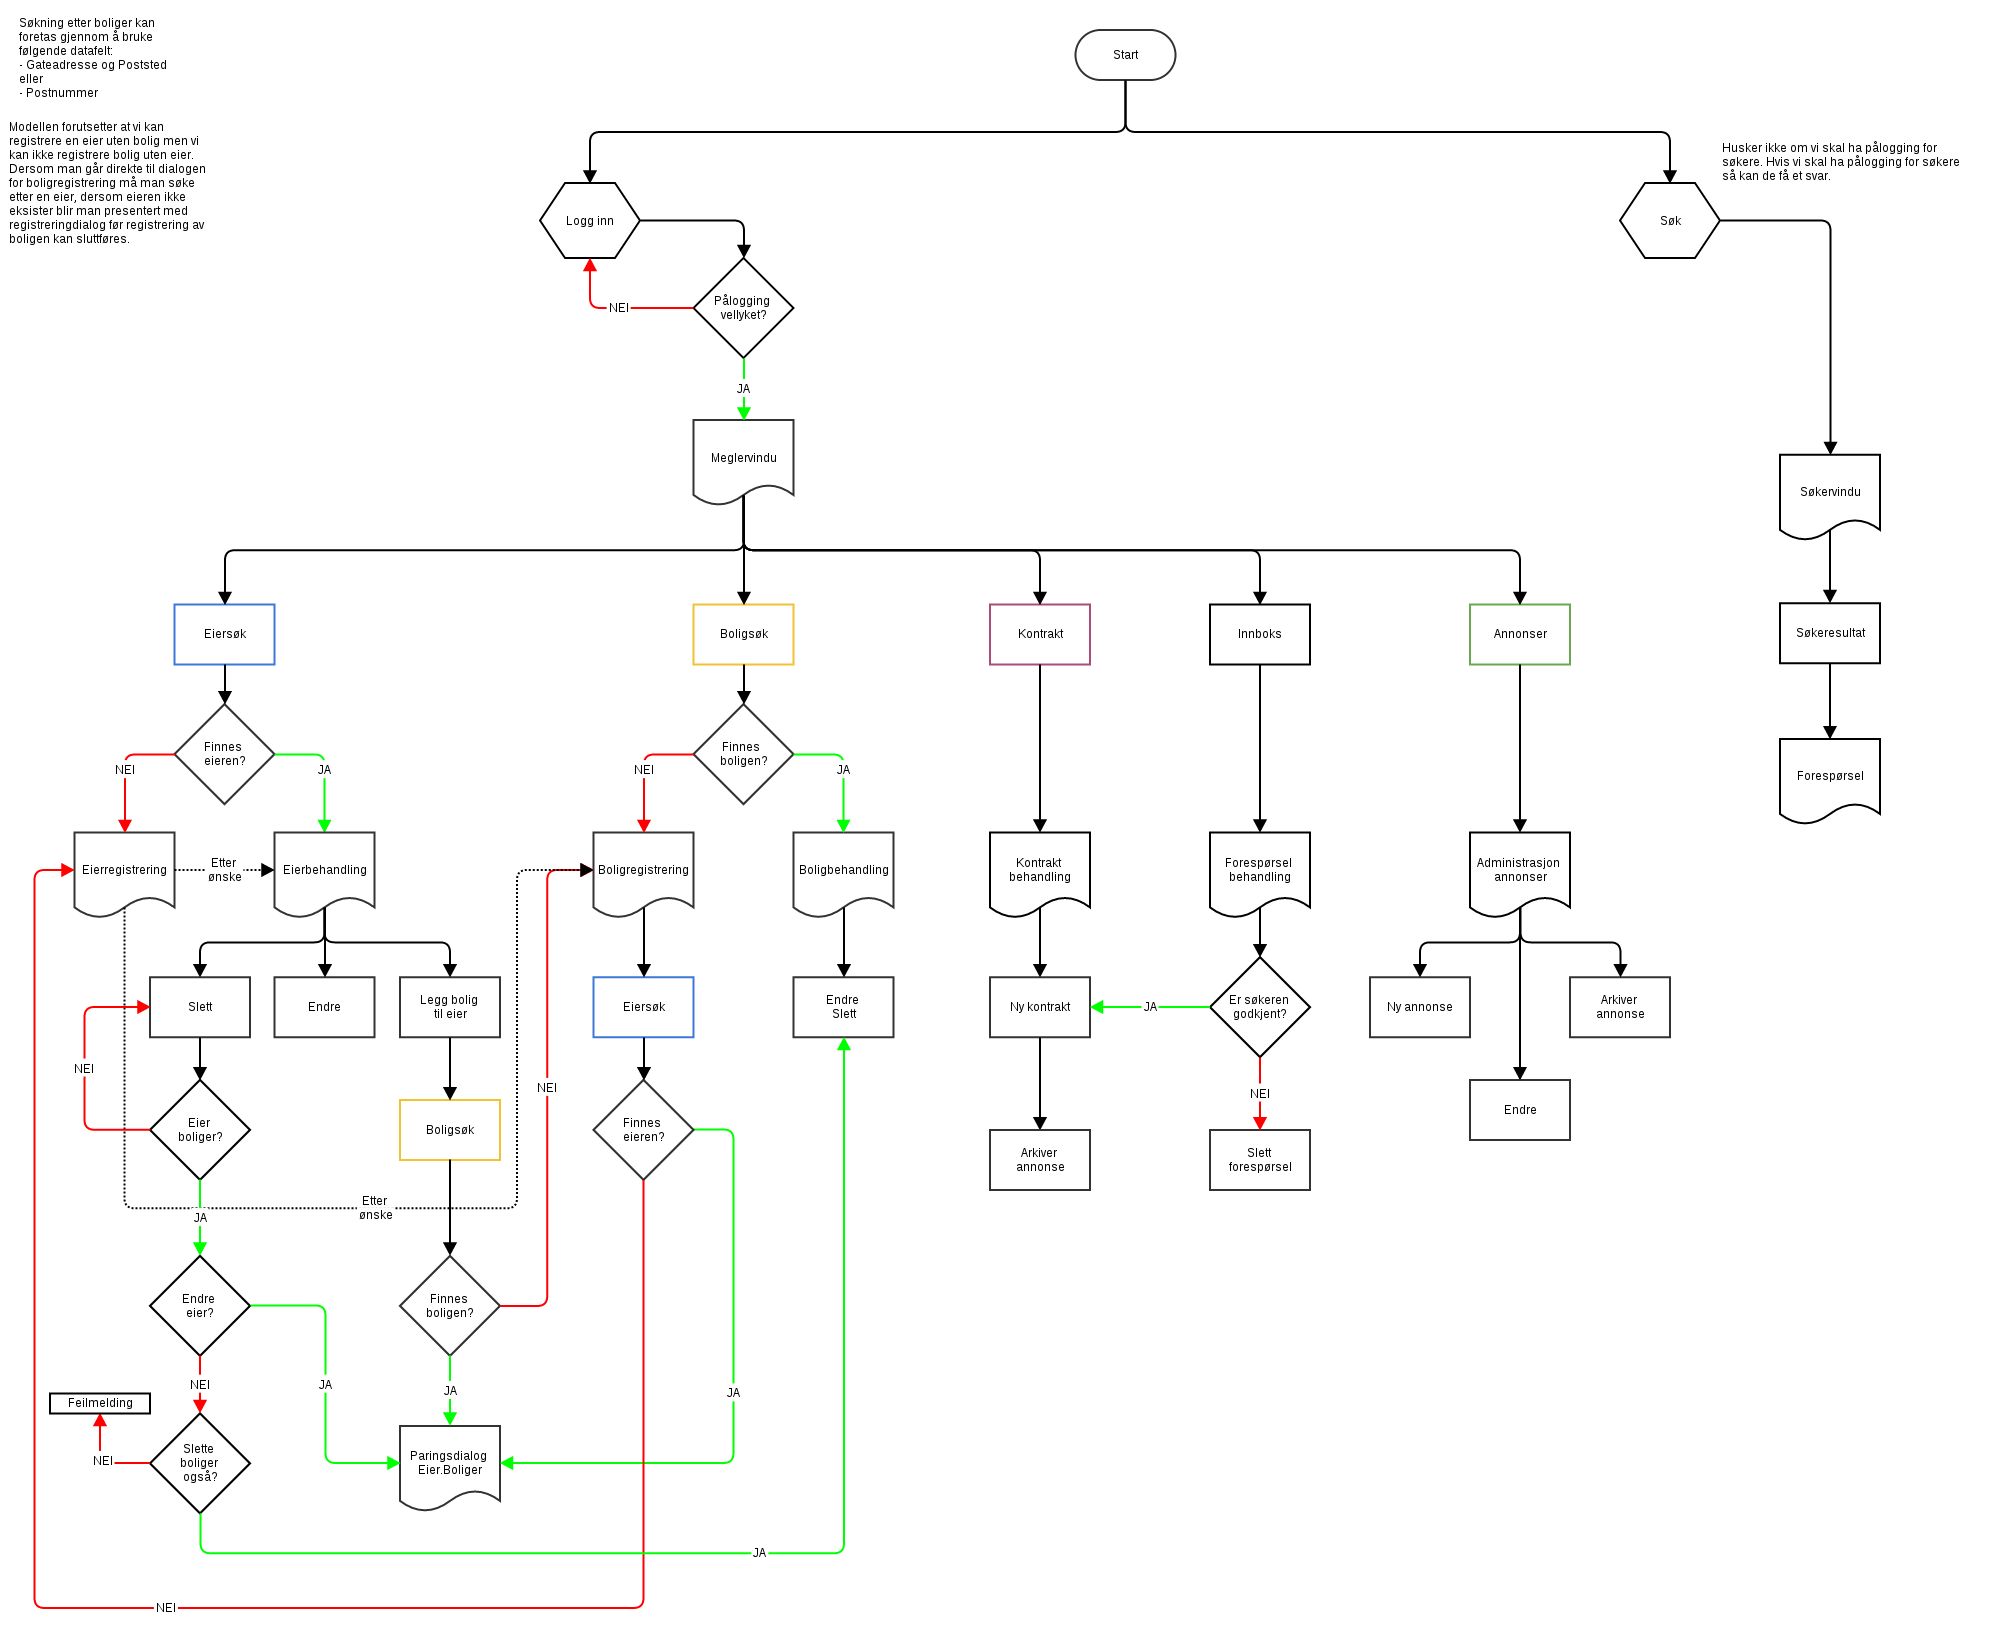
\includegraphics[angle=90 ,width=\textwidth,height=\textheight,keepaspectratio]{./img/appendix/diagram/user_case.png}
 \caption{Flyt diagram over mulig user case som kan foretas i brukergrensesnittet.}
 %Her kommer en kabel for kryssreferering i teksten til figuren
 \label{fig:user_case}
\end{figure}



\begin{figure}[ht]
\begin{center}
 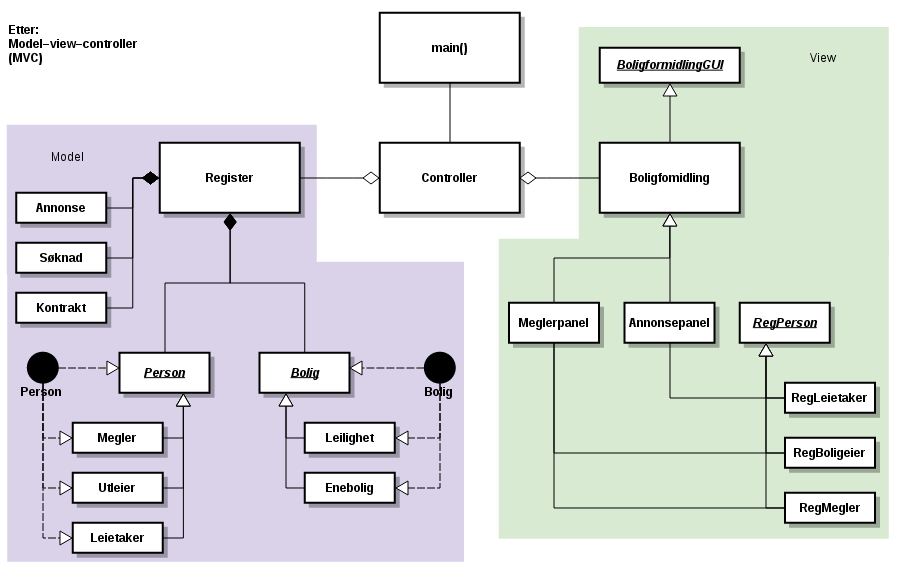
\includegraphics[angle=90, height=21cm]{./img/appendix/diagram/moduler_og_relasjoner.png}
 \caption{Innledende diagram over planlagt MVC arkitektur i programmet.}
 %Her kommer en kabel for kryssreferering i teksten til figuren
 \label{fig:mvc_innledende}
  \end{center}
\end{figure}

\begin{figure}[ht]
\begin{center}
 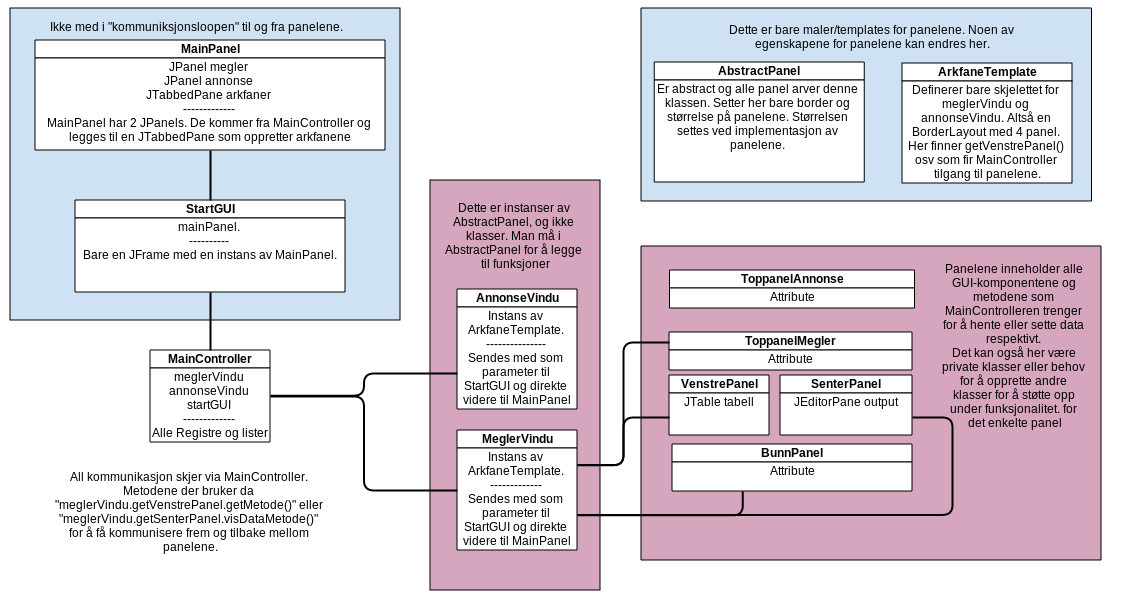
\includegraphics[angle=90, height=21cm]{./img/appendix/diagram/controller_og_gui.png}
 \caption{Flytdiagram over kontroller og GUI klasser.}
 %Her kommer en kabel for kryssreferering i teksten til figuren
 \label{fig:kontroller_og_gui}
 \end{center}
\end{figure}


\begin{figure}[ht]
\begin{center}
 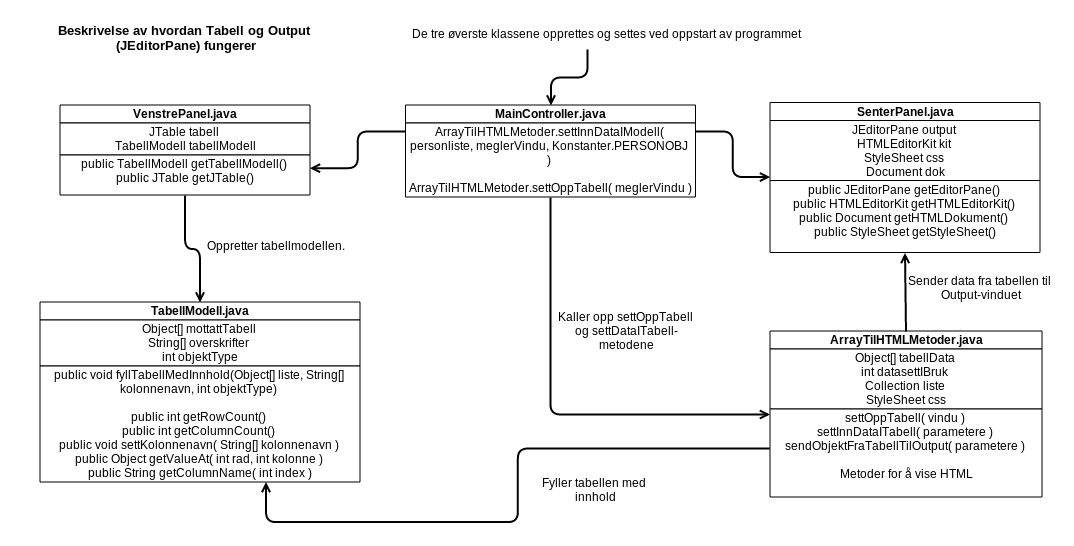
\includegraphics[angle=90 , height=21cm]{./img/appendix/diagram/tabell_og_output.png}
 \caption{Flytdiagram over tabellmodell og output.}
 %Her kommer en kabel for kryssreferering i teksten til figuren
 \label{fig:tabell_og_output}
  \end{center}
\end{figure}
\end{document}
